\documentclass[10pt,review,sigplan,authorversion=true]{acmart}
\settopmatter{printfolios=true,printccs=true,printacmref=true}

\bibliographystyle{ACM-Reference-Format}
\citestyle{acmauthoryear}   %% For author/year citations
\usepackage{listings,multirow,wrapfig,xspace,paralist}
\usepackage{xcolor,tikz,graphicx, pifont}
\usetikzlibrary{positioning,automata,fit,shapes.geometric,backgrounds}

%% \newcommand{\authorcomment}[3]{\xspace\textcolor{#1}{{\bf #2} #3}\xspace}
\newcommand{\authorcomment}[3]{}
% For author notes:
\newcommand{\AG}[1]{\authorcomment{orange}{AG}{#1}}
\newcommand{\JV}[1]{\authorcomment{red}{JV}{#1}}

% For meta comments:
\newcommand{\isit}[1]{\authorcomment{cyan}{Check}{#1}}
\newcommand{\todo}[1]{\authorcomment{red}{TODO}{#1}}
\newcommand{\xmark}{\textcolor{red}{\ding{55}}}
\newcommand{\cmark}{\textcolor{green}{\ding{51}}}

\definecolor{LightGray}{RGB}{247, 247, 247}
\definecolor{Gray}{rgb}{.3,.3,.3}
\definecolor{DarkGray}{rgb}{.5,.5,.5}

\newcommand{\CallCntAsDotenvironment}{10.0M\xspace}
\newcommand{\CallCntAsDotlist}{216.0K\xspace}
\newcommand{\CallCntAsDotlistDotenvironment}{217.0K\xspace}
\newcommand{\CallCntAssign}{392.4K\xspace}
\newcommand{\CallCntBaseenv}{12.2M\xspace}
\newcommand{\CallCntDBrack}{3.6M\xspace}
\newcommand{\CallCntDBrackAssign}{21.1K\xspace}
\newcommand{\CallCntDollar}{2.1M\xspace}
\newcommand{\CallCntDollarAssign}{659.0K\xspace}
\newcommand{\CallCntDotSubsetTwo}{954.4K\xspace}
\newcommand{\CallCntDynget}{2.6K\xspace}
\newcommand{\CallCntEmptyenv}{234.0K\xspace}
\newcommand{\CallCntEnvTwolist}{217.0K\xspace}
\newcommand{\CallCntEnvironment}{13.0M\xspace}
\newcommand{\CallCntEnvironmentAssign}{697.0K\xspace}
\newcommand{\CallCntEnvironmentname}{66.9K\xspace}
\newcommand{\CallCntExists}{505.1K\xspace}
\newcommand{\CallCntGet}{4.9M\xspace}
\newcommand{\CallCntGetZero}{6.1M\xspace}
\newcommand{\CallCntGetnamespace}{6.9M\xspace}
\newcommand{\CallCntGlobalenv}{179.1K\xspace}
\newcommand{\CallCntLength}{375.0\xspace}
\newcommand{\CallCntListTwoenv}{2.6M\xspace}
\newcommand{\CallCntLockbinding}{332.2K\xspace}
\newcommand{\CallCntLockenvironment}{206.2K\xspace}
\newcommand{\CallCntLs}{2.5K\xspace}
\newcommand{\CallCntMget}{291.4K\xspace}
\newcommand{\CallCntNewDotenv}{3.3M\xspace}
\newcommand{\CallCntObjects}{119.0\xspace}
\newcommand{\CallCntParentDotenv}{2.1M\xspace}
\newcommand{\CallCntParentDotenvAssign}{2.2M\xspace}
\newcommand{\CallCntParentDotframe}{6.9M\xspace}
\newcommand{\CallCntPosDottoDotenv}{7.0\xspace}
\newcommand{\CallCntRemove}{14.0K\xspace}
\newcommand{\CallCntRm}{21.1K\xspace}
\newcommand{\CallCntSubstitute}{15.8M\xspace}
\newcommand{\CallCntSysDotcall}{2.2M\xspace}
\newcommand{\CallCntSysDotcalls}{29.2K\xspace}
\newcommand{\CallCntSysDotframe}{6.2M\xspace}
\newcommand{\CallCntSysDotframes}{3.6K\xspace}
\newcommand{\CallCntSysDotfunction}{3.2M\xspace}
\newcommand{\CallCntSysDotnframe}{705.7K\xspace}
\newcommand{\CallCntSysDotparent}{3.8M\xspace}
\newcommand{\CallCntSysDotparents}{7.2K\xspace}
\newcommand{\CallCntTilde}{129.9K\xspace}
\newcommand{\CallCntUnlockbinding}{1.3K\xspace}
\newcommand{\EnvAsnCallPerc}{0.36\xspace}
\newcommand{\EnvAsnCallerName}{MASS::negative.binomial\xspace}
\newcommand{\EnvAsnCoreCallCnt}{114.4K\xspace}
\newcommand{\EnvAsnCoreCallPerc}{48.0\%\xspace}
\newcommand{\EnvAsnCoreFunCnt}{4\xspace}
\newcommand{\EnvAsnCorePackCnt}{2\xspace}
\newcommand{\EnvAsnFiveCallPerc}{0.4\%\xspace}
\newcommand{\EnvAsnFiveCallerName}{\c{MASS::negative.binomial}\xspace}
\newcommand{\EnvAsnFourCallPerc}{3.8\%\xspace}
\newcommand{\EnvAsnFourCallerName}{\c{methods::installClassMethod}\xspace}
\newcommand{\EnvAsnMethodsCallPerc}{75.47\%\xspace}
\newcommand{\EnvAsnOneCallPerc}{50.0\%\xspace}
\newcommand{\EnvAsnOneCallerName}{\c{R6::assign\_func\_envs}\xspace}
\newcommand{\EnvAsnThreeCallPerc}{11.8\%\xspace}
\newcommand{\EnvAsnThreeCallerName}{\c{stats::make.link}\xspace}
\newcommand{\EnvAsnTopFiveCallPerc}{98.59\%\xspace}
\newcommand{\EnvAsnTwoCallPerc}{32.6\%\xspace}
\newcommand{\EnvAsnTwoCallerName}{\c{methods::.makeDefaultBinding}\xspace}
\newcommand{\EnvAsnUnclassifiedCallPerc}{0.05\%\xspace}
\newcommand{\EnvAsnUserCallCnt}{122.9K\xspace}
\newcommand{\EnvAsnUserCallPerc}{52.0\%\xspace}
\newcommand{\EnvAsnUserFunCnt}{37\xspace}
\newcommand{\EnvAsnUserInnerFunCallPerc}{89.58\%\xspace}
\newcommand{\EnvAsnUserInnerFunFunCnt}{21\xspace}
\newcommand{\EnvAsnUserInnerFunPackCnt}{6\xspace}
\newcommand{\EnvAsnUserPackCnt}{17\xspace}
\newcommand{\EnvironmentBaseRegisterMethodCallPerc}{43.8\%\xspace}
\newcommand{\EnvironmentCoreCallCnt}{249.3K\xspace}
\newcommand{\EnvironmentCoreCallPerc}{97\%\xspace}
\newcommand{\EnvironmentCoreFunCnt}{37\xspace}
\newcommand{\EnvironmentCorePackCnt}{5\xspace}
\newcommand{\EnvironmentMethodsCallPerc}{52.2\%\xspace}
\newcommand{\EnvironmentUnclassifiedCallPerc}{0.00\%\xspace}
\newcommand{\EnvironmentUserCallCnt}{6.7K\xspace}
\newcommand{\EnvironmentUserCallPerc}{3\%\xspace}
\newcommand{\EnvironmentUserFunCnt}{33\xspace}
\newcommand{\EnvironmentUserPackCnt}{15\xspace}
\newcommand{\LockBindingCoreCallCnt}{32.1K\xspace}
\newcommand{\LockBindingCoreCallPerc}{9.4\%\xspace}
\newcommand{\LockBindingCoreFunCnt}{3\xspace}
\newcommand{\LockBindingCorePackCnt}{1\xspace}
\newcommand{\LockBindingRSixCallPerc}{89\%\xspace}
\newcommand{\LockBindingUserCallCnt}{309.0K\xspace}
\newcommand{\LockBindingUserCallPerc}{90.6\%\xspace}
\newcommand{\LockBindingUserFunCnt}{7\xspace}
\newcommand{\LockBindingUserPackCnt}{6\xspace}
\newcommand{\LockEnvironmentCoreCallCnt}{166.4K\xspace}
\newcommand{\LockEnvironmentCoreCallPerc}{80.1\%\xspace}
\newcommand{\LockEnvironmentCoreFunCnt}{3\xspace}
\newcommand{\LockEnvironmentCorePackCnt}{1\xspace}
\newcommand{\LockEnvironmentRlangCallCount}{5\xspace}
\newcommand{\LockEnvironmentUserCallCnt}{41.3K\xspace}
\newcommand{\LockEnvironmentUserCallPerc}{19.9\%\xspace}
\newcommand{\LockEnvironmentUserFunCnt}{3\xspace}
\newcommand{\LockEnvironmentUserPackCnt}{2\xspace}
\newcommand{\ObjCntCharacter}{929.9M\xspace}
\newcommand{\ObjCntClosure}{114.0M\xspace}
\newcommand{\ObjCntEnvironment}{1.2B\xspace}
\newcommand{\ObjCntInteger}{453.5M\xspace}
\newcommand{\ObjCntLanguage}{483.9M\xspace}
\newcommand{\ObjCntList}{159.3M\xspace}
\newcommand{\ObjCntLogical}{1.0B\xspace}
\newcommand{\ObjCntOther}{15.2M\xspace}
\newcommand{\ObjCntPromise}{2.8B\xspace}
\newcommand{\ObjCntRaw}{46.4M\xspace}
\newcommand{\ObjCntReal}{113.4M\xspace}
\newcommand{\ObjCntSymbol}{73.5M\xspace}
\newcommand{\ParentFrameCoreCallCnt}{6.0M\xspace}
\newcommand{\ParentFrameCoreCallPerc}{87\%\xspace}
\newcommand{\ParentFrameCoreEightCallPerc}{2.19\%\xspace}
\newcommand{\ParentFrameCoreEightCallerName}{\c{base::new.env}\xspace}
\newcommand{\ParentFrameCoreFiveCallPerc}{7.88\%\xspace}
\newcommand{\ParentFrameCoreFiveCallerName}{\c{base::eval}\xspace}
\newcommand{\ParentFrameCoreFourCallPerc}{12.73\%\xspace}
\newcommand{\ParentFrameCoreFourCallerName}{\c{base::match.call}\xspace}
\newcommand{\ParentFrameCoreFunCnt}{86\xspace}
\newcommand{\ParentFrameCoreNineCallPerc}{1.52\%\xspace}
\newcommand{\ParentFrameCoreNineCallerName}{\c{base::eval.parent}\xspace}
\newcommand{\ParentFrameCoreOneCallPerc}{25.73\%\xspace}
\newcommand{\ParentFrameCoreOneCallerName}{\c{base::delayedAssign}\xspace}
\newcommand{\ParentFrameCorePackCnt}{7\xspace}
\newcommand{\ParentFrameCoreSevenCallPerc}{2.25\%\xspace}
\newcommand{\ParentFrameCoreSevenCallerName}{\c{base::match.fun}\xspace}
\newcommand{\ParentFrameCoreSixCallPerc}{2.65\%\xspace}
\newcommand{\ParentFrameCoreSixCallerName}{\c{base::withCallingHandlers}\xspace}
\newcommand{\ParentFrameCoreTenCallPerc}{1.29\%\xspace}
\newcommand{\ParentFrameCoreTenCallerName}{\c{methods::callNextMethod}\xspace}
\newcommand{\ParentFrameCoreThreeCallPerc}{16.58\%\xspace}
\newcommand{\ParentFrameCoreThreeCallerName}{\c{base::do.call}\xspace}
\newcommand{\ParentFrameCoreTopTenCallPerc}{97.1\%\xspace}
\newcommand{\ParentFrameCoreTwoCallPerc}{24.25\%\xspace}
\newcommand{\ParentFrameCoreTwoCallerName}{\c{base::tryCatch}\xspace}
\newcommand{\ParentFrameDepthOneCallPerc}{83.33\%\xspace}
\newcommand{\ParentFrameDepthOneCallerOneCallPerc}{26.93\%\xspace}
\newcommand{\ParentFrameDepthOneCallerOneCallerName}{\c{base::delayedAssign}\xspace}
\newcommand{\ParentFrameDepthOneCallerTwoCallPerc}{25.39\%\xspace}
\newcommand{\ParentFrameDepthOneCallerTwoCallerName}{\c{base::tryCatch}\xspace}
\newcommand{\ParentFrameDepthOneFunCnt}{432\xspace}
\newcommand{\ParentFrameDepthThreeCallPerc}{0.08\%\xspace}
\newcommand{\ParentFrameDepthThreeCallerOneCallPerc}{70.70\%\xspace}
\newcommand{\ParentFrameDepthThreeCallerOneCallerName}{\c{rlang::caller\_env}\xspace}
\newcommand{\ParentFrameDepthThreeCallerTwoCallPerc}{29.30\%\xspace}
\newcommand{\ParentFrameDepthThreeCallerTwoCallerName}{\c{methods::callNextMethod}\xspace}
\newcommand{\ParentFrameDepthThreeFunCnt}{2\xspace}
\newcommand{\ParentFrameDepthTwoCallPerc}{16.59\%\xspace}
\newcommand{\ParentFrameDepthTwoCallerOneCallPerc}{66.96\%\xspace}
\newcommand{\ParentFrameDepthTwoCallerOneCallerName}{\c{base::match.call}\xspace}
\newcommand{\ParentFrameDepthTwoCallerTwoCallPerc}{11.84\%\xspace}
\newcommand{\ParentFrameDepthTwoCallerTwoCallerName}{\c{base::match.fun}\xspace}
\newcommand{\ParentFrameDepthTwoFunCnt}{21\xspace}
\newcommand{\ParentFrameUserCallCnt}{877.5K\xspace}
\newcommand{\ParentFrameUserCallPerc}{13\%\xspace}
\newcommand{\ParentFrameUserEightCallPerc}{3.07\%\xspace}
\newcommand{\ParentFrameUserEightCallerName}{\c{glue::glue}\xspace}
\newcommand{\ParentFrameUserFiveCallPerc}{5.38\%\xspace}
\newcommand{\ParentFrameUserFiveCallerName}{\c{rlang::enquo}\xspace}
\newcommand{\ParentFrameUserFourCallPerc}{7.84\%\xspace}
\newcommand{\ParentFrameUserFourCallerName}{\c{rlang::enexpr}\xspace}
\newcommand{\ParentFrameUserFunCnt}{360\xspace}
\newcommand{\ParentFrameUserNineCallPerc}{2.66\%\xspace}
\newcommand{\ParentFrameUserNineCallerName}{\c{ggplot2::ggproto}\xspace}
\newcommand{\ParentFrameUserOneCallPerc}{25.57\%\xspace}
\newcommand{\ParentFrameUserOneCallerName}{\c{withr::defer}\xspace}
\newcommand{\ParentFrameUserPackCnt}{81\xspace}
\newcommand{\ParentFrameUserSevenCallPerc}{3.95\%\xspace}
\newcommand{\ParentFrameUserSevenCallerName}{\c{testthat::R6(Reporter)::local\_user\_output}\xspace}
\newcommand{\ParentFrameUserSixCallPerc}{5.33\%\xspace}
\newcommand{\ParentFrameUserSixCallerName}{\c{vctrs::s3\_register}\xspace}
\newcommand{\ParentFrameUserTenCallPerc}{2.09\%\xspace}
\newcommand{\ParentFrameUserTenCallerName}{\c{rlang::defer}\xspace}
\newcommand{\ParentFrameUserThreeCallPerc}{12.79\%\xspace}
\newcommand{\ParentFrameUserThreeCallerName}{\c{rlang::caller\_env}\xspace}
\newcommand{\ParentFrameUserTopTenCallPerc}{82.5\%\xspace}
\newcommand{\ParentFrameUserTwoCallPerc}{13.76\%\xspace}
\newcommand{\ParentFrameUserTwoCallerName}{\c{rlang::captureArgInfo}\xspace}
\newcommand{\UnlockBindingCoreCallCnt}{688.0\xspace}
\newcommand{\UnlockBindingCoreCallPerc}{53.8\%\xspace}
\newcommand{\UnlockBindingCoreFunCnt}{1\xspace}
\newcommand{\UnlockBindingCorePackCnt}{1\xspace}
\newcommand{\UnlockBindingUserCallCnt}{590.0\xspace}
\newcommand{\UnlockBindingUserCallPerc}{46.2\%\xspace}
\newcommand{\UnlockBindingUserFunCnt}{5\xspace}
\newcommand{\UnlockBindingUserPackCnt}{5\xspace}


%% https://www.davehofmann.de/defining-custom-language-templates-for-latex-listings/
% Define Language
\lstdefinelanguage{smalleR} {
  % list of keywords
  morekeywords={
    for,
    if,
    else,
    function
  },
  sensitive=true, % keywords are not case-sensitive
  morecomment=[l]{\#}, % l is for line comment
  morestring=[b]{"} % defines that strings are enclosed in double quotes
}

\lstset{
  language={smalleR},
  columns=flexible,
  captionpos=b,
  frame=single,
  framerule=0pt,
  framexleftmargin=1mm,
  framexrightmargin=1mm,
  tabsize=2,
  belowskip=0pt,
  basicstyle=\small\ttfamily,
  backgroundcolor=\color{LightGray},
  emphstyle=\sffamily,
  keywordstyle=\bfseries,
  commentstyle=\color{Gray}\em,
  stringstyle=\color{Gray},
  alsoletter={., _, $},
  breaklines=true
}

\newcommand{\code}[1]{\lstinline |#1|\xspace}
\renewcommand{\c}[1]{\lstinline |#1|\xspace}
\newcommand{\eg}{\emph{e.g.},\xspace}
\newcommand{\ie}{\emph{i.e.},\xspace}

\newcommand{\environmentFun}{\code{environment}}
\newcommand{\asEnvironment}{\code{as.environment}}

\newcommand{\emptyenv}{\code{empyenv}}
\newcommand{\globalenv}{\code{globalenv}}

\newcommand{\base}{\code{base}}
\newcommand{\methods}{\code{methods}}
\newcommand{\lazyLoadDBexec}{\code{lazyLoadDBexec}}

\newcommand{\newEnv}{\code{new.env}}

\newcommand{\asList}{\code{as.list}}
\newcommand{\listToEnv}{\code{list2env}}

\newcommand{\ls}{\code{ls}}
\newcommand{\objects}{\code{objects}}

\newcommand{\subDollar}{\code{$}}
\newcommand{\subBracket}{\code{[[}}

\newcommand{\exist}{\code{exist}}

\newcommand{\get}{\code{get}}
\newcommand{\getZero}{\code{get0}}
\newcommand{\mget}{\code{mget}}
\newcommand{\dynGet}{\code{dynGet}}

\newcommand{\assign}{\code{assign}}

\newcommand{\remove}{\code{remove}}
\renewcommand{\rm}{\code{rm}}

\newcommand{\lockEnvironment}{\code{lockEnvironment}}
\newcommand{\lockBinding}{\code{lockBinding}}
\newcommand{\unlockBinding}{\code{unlockBinding}}

\newcommand{\eval}{\code{eval}}
\newcommand{\substitute}{\code{substitute}}

\newcommand{\parentEnv}{\code{parent.env}}
\newcommand{\parentEnvAssign}{\code{parent.env<-}}

\newcommand{\envtracer}{{\sf envtracer}\xspace}
\newcommand{\experimentr}{{\sf experimentr}\xspace}
\newcommand{\rdyntrace}{{\sf R-dyntrace}\xspace}

\newcommand{\ggplot}{\textit{ggplot2}\xspace}
\newcommand{\vctrs}{\textit{vctrs}\xspace}

%%% \setcopyright{rightsretained}
%%% \acmPrice{}
%%% \acmDOI{10.1145/3360579}
%%% \acmYear{2019}
%%% \copyrightyear{2019}
%%% \acmJournal{PACMPL}
%%% \acmVolume{3}
%%% \acmNumber{OOPSLA}
%% \acmArticle{153}
%%% \acmMonth{10}
\begin{document}
\title{First-Class Environments in R}
\author{Aviral Goel}\affiliation{\institution{Northeastern University}\country{}}
\author{Jan Vitek}\affiliation{\institution{Czech Technical University in Prague\\Northeastern University}\country{}}
\authorsaddresses{}
\renewcommand{\shortauthors}{Goel, Vitek}


\begin{abstract}
  The R programming language is widely used for statistical computing. To enable
  interactive data exploration and rapid prototyping, R encourages a dynamic
  programming style. This programming style is supported by features such as
  first-class environments. Amongst widely used languages, R has the richest
  interface for programmatically manipulating environments. With the flexibility
  afforded by reflective operations on first-class environments, come
  significant challenges for reasoning and optimizing user-defined code. This
  paper documents the reflective interface used to operate over first-class
  environment. We explain the rationale behind its design and conduct a large
  scale study of how the interface is used in popular libraries.
\end{abstract}

\begin{CCSXML}
<ccs2012>
<concept>
<concept_id>10002944.10011123.10010912</concept_id>
<concept_desc>General and reference~Empirical studies</concept_desc>
<concept_significance>500</concept_significance>
</concept>
<concept>
<concept_id>10011007.10011006.10011008</concept_id>
<concept_desc>Software and its engineering~General programming languages</concept_desc>
<concept_significance>500</concept_significance>
</concept>
<concept>
<concept_id>10011007.10011006.10011050.10010517</concept_id>
<concept_desc>Software and its engineering~Scripting languages</concept_desc>
<concept_significance>500</concept_significance>
</concept>
<concept>
<concept_id>10011007.10011006.10011039.10011311</concept_id>
<concept_desc>Software and its engineering~Semantics</concept_desc>
<concept_significance>300</concept_significance>
</concept>
</ccs2012>
\end{CCSXML}

\ccsdesc[500]{General and reference~Empirical studies}
\ccsdesc[500]{Software and its engineering~General programming languages}
\ccsdesc[500]{Software and its engineering~Scripting languages}
\ccsdesc[300]{Software and its engineering~Semantics}

%\keywords{R language, delayed or lazy evaluation}

\maketitle
\section{Introduction}

The ability to name values is a building block of linguistic abstractions. Local
variables, global variables, function parameters, all boil down to a mapping
from names to values, commonly referred to as an \emph{environment}. The
semantics of environments have a profound impact on how languages can be
implemented. At a first approximation, the more restricted the semantics, the
easier it is to implement the language efficiently. Early languages did not
support recursion, thus their compilers could generate code where each variable
had its unique, pre-determined, location in the computer's memory. When a
variable's value was determined to be constant, it did not even need a memory
location, the variable was effectively an alias for that value. As languages
became more expressive, implementations had to store variables in data
structures such as the stack, for traditional imperative languages, or in
heap-allocated records, for functional languages. When the compiler could assume
all variable accesses were known at compile time, the variables could be
represented by offsets from a known location. On the the other hand, for
languages that allowed symbolic lookups, the mapping between names and locations
had to be retained. Each of these choices comes with performance implications.

The R programming language was created in 1993~\cite{r96} as a direct descendent
to S whose origin dates to 1976~\cite{s88}. Both languages found inspiration in
earlier work on Lisp~\cite{Lisp}, CLOS~\cite{CLOS}, and
Scheme~\cite{SchemeR5RS}. Yet, they chose to depart from those previous
languages in small and large ways. R evolved to become a functional language,
without type annotations, with delayed evaluation of function arguments, mutable
state, and various mechanisms for supporting object-oriented programming.

At heart, R is a simple language. Its expressivity stems from the combination of
delayed evaluation and the language's rich reflective interface that allows to
extend the core semantics in various ways. One of the keys design choices was to
make environments first-class and allow full programmatic access over
environments.

In R, an environment is an unordered mutable map from symbols to values.
Environments are omnipresent -- they represent name spaces, or scopes, for
variables within a function, but also the name spaces that are constructed when
a package is loaded. As they are the only mutable data structure in the language
they are also used as hashmaps and objects. They are created implicitly when a
function is called, and explicitly with \c{new.env}. Operations are provided to
read variables and update or delete them. It is even possible change the
association between a closure and its environment. R's interface allows, for
example, to acquires the environment of the caller of the currently executing
function, check if it contains a variable \c{x}, and rename it to \c{y}.
Needless to say that this flexibility causes headaches to implementers,
\citet{dls19} gives an account of these challenges.

This paper documents the interface that R exposes to environments. This
interface evolved through the years. It is rich and not always consistent, and
certainly not minimal. Through a dynamic analysis conducted on a corpus of
popular R libraries and their clients, we report on the practical usage of
environments. This allows us to explain the need for this interface and could,
possibly, be a step towards a re-design or a warning for compiler writers.

\vspace{2mm}

\noindent Our implementation is available from \url{FINALIZE}.

\newpage

\section{Related Work}

Imperative languages like C or Fortran have tried to have efficient
implementations of environments, typically variables are encoded by offsets from
a stack pointer and symbolic references are only allowed during debugging of
non-optimized code. Statically typed functional languages have first-class
functions and thus must allocate environments on the heap, but they usually
retain the variable-as-offset implementation technique.

More dynamic languages must retain more information at run-time. For example, to
support dynamic code generation through the \c{eval} function, it is necessary
to retain the mapping between symbols and locations. When the language allows to
programmatically add and remove variables, most hope for an efficient
compilation strategy dies. Different languages make various choices. The Scheme
Standard specifies that \code{eval} takes an environment-specifier, which needs
not be a first-class environment~\cite{SchemeR5RS}. The effect of assignment to
variables in this environment is unspecified, leaving open the possibility of it
being immutable. Scheme supports first-class environments and, as a consequence,
its \code{eval} takes an explicit environment. It provides functions to create
new environments, read and write bindings, examine parent environments, and
obtain the current environment as a reified value. Python provides the
\code{locals} function that returns the local bindings as a dictionary, attached
to the current frame as an attribute. Updates to this dictionary are not
reflected in the function's scope. Caller's bindings can be accessed from their
frame obtained by calling \code{inspect.stack}. Calling \code{locals} outside of
a function returns the namespace as a dictionary at the point and changes to
this dictionary are reflected in the namespace. Python's \code{globals} returns
a dictionary of the global namespace whose updates are also reflected in the
namespace~\cite{}.

\citet{NishizakiSTLC94} introduced a simply typed lambda calculus with
first-class environments, proved that it is strongly normalizing, and proposed a
type inference algorithm. \citet{NishizakiML94} proposed a sound type inference
algorithm for a type system with ML-polymorphism in a $\lambda$-calculus with
first-class environments. Their language has \c{the-environment} function for
reifying the current environment and \c{eval} for evaluating an expression in an
environment.

\citet{ecoop12} discussed the design of R, providing a comprehensive explanation
of R's scoping and evaluation mechanism. They present many aspects of
environments in the context of laziness, metaprogramming, dynamic evaluation,
explicit environment manipulation, and call stack inspection, but they don't
discuss explicit environment creation using \code{new.env}. In comparison to
their work, our work focuses only on environments and provides a much more
detailed qualitative and quantitative account. Furthermore, our study shows a
significantly larger and richer use of explicit environments in the R ecosystem
compared to theirs. \citet{oopsla19b} studied the design and use of laziness in
R. They provide a detailed account of the language’s evaluation strategy with a
small-step operational semantics and an empirical evaluation of laziness in
16,707 packages. Their semantics shows that promises are stored in environments
and can outlive the frame that created them if returned as part of that
environment. \citet{oopsla20b} inferred type signatures for R functions by
observing the type of argument and return values. Their type language includes a
type for first-class environments.


\section{The R language}

A presentation of the language requires introducing some key concepts. We will
be brief, interested readers should consult~\cite{AdvancedR}.

\paragraph{Functions} Functions are first-class, anonymous, lexically-scoped values
with optional parameters and default values. R is ``functional'' in the sense
that values have a copy-on-write semantics, so side-effects to arguments inside
a function are not reflected to the caller.

\paragraph{Promises} R is a mostly lazy language. Arguments to functions are
packaged into promises which bundle an expression and its environment. When the
value of a promise is needed, the expression is evaluated in the adjoined
environment and the result is cached in the promise.

\paragraph{Vectors}  Most values in R are vectors, and most operations are
vectorized. Vectors are homogeneous arrays of integer, double, character,
logical, complex, or raw values.

\paragraph{Lists} Lists are heterogeneous vectors with optionally named elements.
They can be indexed by position or name. Lists (and vectors) have a
copy-on-write semantics.

\paragraph{Attributes}
Values can be tagged with user-defined attributes which are a map from string to
value. Consider the following code which sets the attributes \code{dim} and
\c{class} of some vector \code{x}.

\begin{lstlisting}
  x <- c(1,2,3,4)
  attr(x, dim) <- c(2,2)
  class(x) <- c("cat")
\end{lstlisting}
\noindent
Setting the \code{dim} attribute causes the vector to be subsequently treated as
a 2$\times$2 matrix. Similarly, the class attribute is used for method dispatch
in an object-oriented style.

\paragraph{Formulas}  A formula is a compact symbolic representation of models
used by statistical functions. For example, the linear model \code{y~x-1}
specifies a line through the origin. Each formula contains a reference to the
environment in which it is defined to refer to the variables, if they are not
otherwise provided during model fitting.

\section{Environments in R}

The evolution of R has been gradual, rather a panoply of abstractions, the
language designer opened up the internals of the interpreter for all to see, and
packaged some commonly needed functionality with the core of the language. Thus,
the task of describing the ``interface'' of environments as seen by developers
and end-users involves some sleuthing. As we prepared this paper, we kept
discovering new functions that accessed environments from native code. This
section is not meant to be an exhaustive, but it gives an overview of the most
commonly used functions.

Environments are implemented either by an association list or a hashmap, as
specified by construction parameter. Each environment also has a parent, forming
an acyclic chain terminated by the empty environment. That environment is
returned by \code{emptyenv()}. Unlike other values, environments are mutable.

\subsection{Environments as Packages}

Packages are loaded by calls to the \code{library()} function, and are
represented by environments; their names are added to a global search path.
Package can be retrieved by position, the \emph{n}-th package is
\code{as.environment(n)} or by name. Every package has a corresponding namespace
which contains its private bindings and implementation specific metadata. A
namespace can be obtained by calling \code{getNamespace(p)}. \code{baseenv()}
returns the base package environment that is pre-loaded witih R and binds
\code{.BaseNamespaceEnv} to it.


\subsection{Environments as Lexical Scopes}

In R, each function has a lexical scope. Furthermore each nested function
introduces a nested scope. When a function begins executing, its scope is
initialized with parameters, and, as it runs, new variables are introduced
implicitly each time an undefined symbol is assigned to. R allows to obtain the
current scope with a call to \code{environment()}. From there it is possible to
read and update the environment through the reference returned by that function.

R provides access to the call stack. Frames starts from 0 and increases by one
for each nested call. Function \code{sys.nframe} returns the current frame
number, and \code{sys.parent(n)} returns the number of the \code{n}th parent.
The function \code{sys.frame(n)} returns environment at that position (counting
backwards if \code{n} is negative); \code{parent.frame(n)} optimises calls to
\code{sys.frame(sys.parent(n))}. Lastly, \code{sys.frames()} returns a list of
active environments.

\begin{lstlisting}
 f <- function() { print(environment()); g() }
 g <- function() { print(parent.frame(1)); }
 f()
 # <env: 0x7f2> <env: 0x7f2>
\end{lstlisting}

\noindent
In the above code snippet, \c{f} accesses its own environment using the call to
\c{environment()} and it's callee \c{g} accesses \c{f}'s environment by calling
\c{parent.frame(-1)}.

The global environment , referred by the variable \code{.GlobalEnv} (at offset
0), is returned by \code{globalenv()}. One can rebind the enclosing environment
of a function with \code{environment(f)<-e}.

\begin{lstlisting}
 f <- function() print(environment())
 environment(); environment(f); f()
 # <env: Global> <env: Global> <env: 0x7ff>
 e <- new.env()
 print(e)
 # <env: 0x7f1>
 environment(f) <- e
 environment(f)
 # <env: 0x7f1>
\end{lstlisting}

The code snippet above modifies the enclosing scope of \c{f}, defined at the
top-level. The environment \c{e}, created using \c{new.env}, is assigned the
enclosing scope of \c{f} using \c{environment(f) <- e}.

\begin{figure*}[t!]
 \centering
 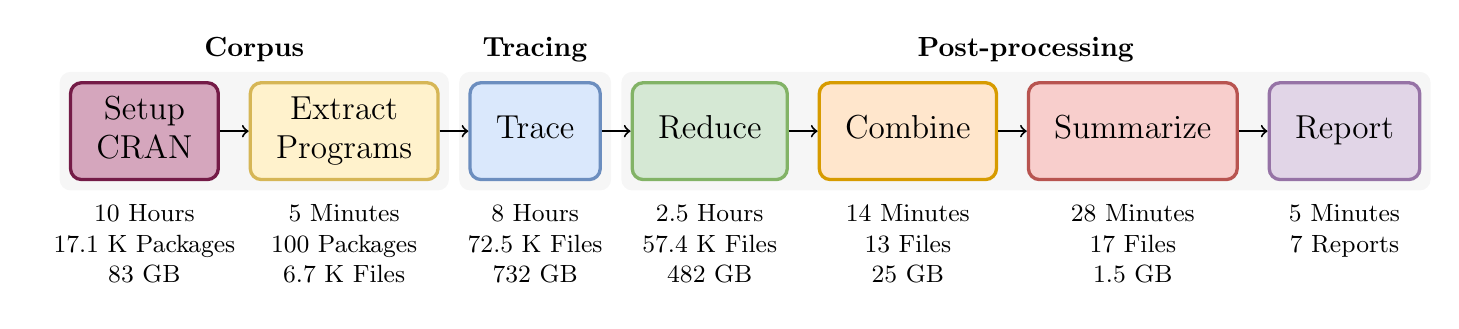
\begin{tikzpicture}
  \definecolor{maroon}{HTML}{D5A6BD}
  \definecolor{darkmaroon}{HTML}{741B47}
  \definecolor{yellow}{HTML}{FFF2CC}
  \definecolor{darkyellow}{HTML}{D6B656}
  \definecolor{blue}{HTML}{DAE8FC}
  \definecolor{darkblue}{HTML}{6C8EBF}
  \definecolor{green}{HTML}{D5E8D4}
  \definecolor{darkgreen}{HTML}{82B366}
  \definecolor{orange}{HTML}{FFE6CC}
  \definecolor{darkorange}{HTML}{D79B00}
  \definecolor{red}{HTML}{F8CECC}
  \definecolor{darkred}{HTML}{B85450}
  \definecolor{purple}{HTML}{E1D5E7}
  \definecolor{darkpurple}{HTML}{9673A6}
  \definecolor{gray}{HTML}{F5F5F5}
  \newcommand{\nodesep}[0]{0.030 \textwidth}
  \newcommand{\textsep}[0]{0.010 \textwidth}
  \newcommand{\backopacity}[0]{0.9}
  \newcommand{\nodename}[1]{\large \begin{tabular}{c}#1\end{tabular}}
  \newcommand{\nodedesc}[1]{\small \begin{tabular}{c}#1\end{tabular}}
  \tikzstyle{block}     = [rectangle, rounded corners, minimum width=.08 \textwidth, minimum height=35pt]
  \tikzstyle{connector} = [line width=0.25mm, ->]
  \node [block, draw = darkmaroon, very thick, fill = maroon]                                (install)   {\nodename{Setup\\CRAN}};
  \node [block, draw = darkyellow, very thick, fill = yellow, right = \nodesep of install  ] (extract)   {\nodename{Extract\\Programs}};
  \node [block, draw = darkblue,   very thick, fill = blue  , right = \nodesep of extract  ] (trace)     {\nodename{Trace}};
  \node [block, draw = darkgreen,  very thick, fill = green , right = \nodesep of trace    ] (reduce)    {\nodename{Reduce}};
  \node [block, draw = darkorange, very thick, fill = orange, right = \nodesep of reduce   ] (combine)   {\nodename{Combine}};
  \node [block, draw = darkred,    very thick, fill = red   , right = \nodesep of combine  ] (summarize) {\nodename{Summarize}};
  \node [block, draw = darkpurple, very thick, fill = purple, right = \nodesep of summarize] (report)    {\nodename{Report}};
  \draw [connector] (install)   edge (extract);
  \draw [connector] (extract)   edge (trace);
  \draw [connector] (trace)     edge (reduce);
  \draw [connector] (reduce)    edge (combine);
  \draw [connector] (combine)   edge (summarize);
  \draw [connector] (summarize) edge (report);
  \node [below = \textsep of install]   (installdesc)   {\nodedesc{10 Hours\\17.1 K Packages\\83 GB}};
  \node [below = \textsep of extract]   (extractdesc)   {\nodedesc{5 Minutes\\100 Packages\\6.7 K Files}};
  \node [below = \textsep of trace]     (tracedesc)     {\nodedesc{8 Hours\\72.5 K Files\\732 GB}};
  \node [below = \textsep of reduce]    (reducedesc)    {\nodedesc{2.5 Hours\\57.4 K Files\\482 GB}};
  \node [below = \textsep of combine]   (combinedesc)   {\nodedesc{14 Minutes\\13 Files\\25 GB}};
  \node [below = \textsep of summarize] (summarizedesc) {\nodedesc{28 Minutes\\17 Files\\1.5 GB}};
  \node [below = \textsep of report]    (reportdesc)    {\nodedesc{5 Minutes\\7 Reports}};
    \begin{scope}[on background layer]
    \node[fit=(install) (extract), rectangle, rounded corners, fill=gray, fill opacity=\backopacity, label=above:\textbf{Corpus}]          (corpus) {};
    \node[fit=(trace),             rectangle, rounded corners, fill=gray, fill opacity=\backopacity, label=above:\textbf{Tracing}]         (exectrace) {};
    \node[fit=(reduce) (report),   rectangle, rounded corners, fill=gray, fill opacity=\backopacity, label=above:\textbf{Post-processing}] (postprocessing) {};
  \end{scope}
 \end{tikzpicture}
  \caption{Analysis Pipeline}\label{fig:analysisPipeline}
\end{figure*}


\subsection{Environments as Data Structures}

Environments can be created using the \newEnv function. This function takes
three optional arguments: a boolean to select a hash table representation over
the default association list, a size for preallocation, and, an enclosing
environment. R does not provide any function to query the representation used
for an environment. The \code{length} function returns the number of bindings in
an environment. \parentEnv yields the enclosing environment and
\code{parent.env(e)<-p} sets the enclosing environment of \code{e} to \code{p}.

\begin{lstlisting}
  e <- new.env(parent=emptyenv())
  length(e)
  # 0
  parent.env(e)
  # <environment: R_EmptyEnv>
  parent.env(e) <- globalenv()
  parent.env(e)
  # <environment: R_GlobalEnv>
\end{lstlisting}

\asList converts environments to lists; in R lists can associate names with
elements. \listToEnv copies the elements of a list to an environment. If the
environment is not supplied, it creates one using \newEnv. The variables of an
environment can be retrieved as a vector using the \ls and \objects functions.

\begin{lstlisting}
  l <- list(x=1, y=2); e <- list2env(l)
  length(e)
  # 2
  as.list(e)
  # list(y = 2, x = 1)
  ls(e)
  # [1] "x" "y"
\end{lstlisting}

\noindent
A variable's existence in an environment can be queried using \exist. Its value
can be retrieved using \subDollar and \subBracket operators. \get, \getZero,
\mget, and \dynGet functions are generalizations of these operators with options
to perform lookup recursively in parent environments (\code{inherits = TRUE})
and validate the type of value bound to the variable being read (\code{mode =
  "integer"}). \getZero is \get with an extra argument, \code{ifnotfound}, which
is returned if the variable is not present in the environment. \mget is a
vectorized version of \get; it reads multiples variables supplied as a vector
and returns a vector of values. \dynGet performs recursive lookups in caller
frames, i.e., dynamic scopes, unlike the other functions which perform lookups in
lexical scopes.

Writes can be performed in an environment using the \assign function. Operator
forms, \code{env$var <- val}, and \code{env[["var"]] <- val}, can also be used
for mutating variable \code{var} in environment \code{env}. Bindings
can be removed from an environment using the \rm and \remove function.

An environment can be protected from the addition or removal of bindings by
locking it with \lockEnvironment. This does not protect existing bindings from
modification, which can be explicitly locked using \lockBinding. A locked
binding can be removed if the environment is not locked. Bindings can be
unlocked using \unlockBinding.

Expressions can be evaluated explicitly in an environment using the \eval
function. To support metaprogramming, R provides the \substitute function. This
function extracts the unevaluated argument text from the promise bound to the
argument in the supplied environment.


\section{Infrastructure and Corpus}

The experimental results reported in this paper are produced by a dynamic
analysis infrastructure running over a large corpus of R programs. The
infrastructure has three tasks: assembling executable programs from R packages,
generating execution traces using a modified R interpreter, and post-processing
the traces to generate graphs and statistics. For reproducibility, the
infrastructure lives in a Docker container based on Debian 10.9.
Figure~\ref{fig:analysisPipeline} summarizes the pipeline along with the
duration of each stage and the size of returned results.

\subsection{A Corpus of R Programs}

Our corpus is assembled from R packages hosted on CRAN \cite{ligges2017}, the
official R package repository. We mirror CRAN on our server and install its
packages. We downloaded and installed 17,133 CRAN packages.\footnote{Snapshot
taken on 29 May 2021.} From these, we select the 100 CRAN packages with highest
number of clients. These 100 packages together have 11,786 clients (\ggplot has
the highest number of clients, 2,320, and package \vctrs has the fewest, 108).
These packages contain 481K lines of R code and 1M lines of native code. During
execution, these 100 packages call functions from 186 other packages, so our
evaluation also includes them. These extra packages have 478K lines of R code
and 1.1M lines of native code.

CRAN packages come equipped with runnable code in the form of tests, examples,
and long-form examples called vignettes. These programs are extracted as
independently executable scripts for evaluation by the \experimentr library. (=
= = ADD CITE= = =) Experiments demonstrate the use of a package's functions, and
vignettes illustrate a package's functionality with a larger example, typically
using data supplied with the package. Overall, there are 6.9K scripts with
205.8K lines of code, Table~\ref{table:corpus} has details.

\begin{table}[!h]  \vspace{-3mm}  \small  \centering
  \caption{Corpus}\label{table:corpus}
  \vspace{-3mm}
  \begin{tabular}{lrrr}    \toprule
    &\bf Tests&\bf Examples&\bf Vignettes\\    \midrule
    {Scripts}&1.9K&5.0K&187.0\\    \midrule
    {LOC}&136.7K&55.2K&13.9K\\
    \bottomrule
  \end{tabular}
\end{table}

\subsection{Dynamic Analysis of R}

Execution traces are generated using \envtracer, a dynamic analyzer built on top
of \rdyntrace. \rdyntrace modifies GNU R 4.0.2~\cite{oopsla19b} to record events
during program execution. We use these callbacks to collect execution
information associated with environments. The events include function entry and
exit, eval entry and exit, object allocation and deallocation, package loading
and attaching, variable lookup, assignment, and removal, subassignment,
subsetting, and attribute setting. When the program exits, \envtracer stores the
traces in a tabular format. To handle the subtleties of R, \envtracer maintains
models of concrete R objects, such as environments, functions, calls, and frames
on the call stack. Model objects have unique identities, whereas R objects are
identified by their memory address, and the garbage collector can reuse these.
\envtracer heuristically constructs names of model functions. The model stack
updates itself appropriately in response to longjump used by R for non-local
returns.

\subsection{Post-processing Traces}

The execution traces must be analyzed to gather insights. \envtracer gathers
681GB of data, scale is thus the major challenge. We use a custom map-reduce
analysis that first processes individual traces in parallel to generate smaller
tables per program. This is expensive but it substantially reduces data size.
Then the tables are concatenated into a single table per analysis. Finally
summaries are computed from the concatenated tables. The report phase generate
graphs and tables from these summaries.

\section{How Frequent are Environments?}

The 286 corpus packages have 44K functions, of which 18K are exercised. From the
un-exercised 25K functions, the majority belong to transitively included
packages for which we do not have tests, and, some 8K functions are from our
initial target packages but were unused. Table~\ref{table:packsize} presents the
distribution of exercised functions across these packages. We observe that 171
packages have 25 functions or less. There are few large packages; 8 with more
than 500 functions.

\begin{table}[!h]  \vspace{-2mm}  \small
  \caption{Package Size} \label{table:packsize}  \centering
  \begin{tabular}{lr}    \toprule
    \bf Functions&\bf Packages\\    \midrule
    1--25&169\\
    26--50&40\\
    51--100&17\\
    101--150&14\\
    151--200&11\\
    201--250&15\\    \bottomrule
  \end{tabular}
  \quad
  \begin{tabular}{lr}    \toprule
    \bf Functions&\bf Packages\\    \midrule
    251--300&4\\
    301--400&6\\
    401--500&2\\
    501--600&3\\
    601--700&0\\
    701--800&3\\    \bottomrule
  \end{tabular}
\end{table}

\noindent
We observed 42M calls to these functions. Figure~\ref{fig:calldist} shows the
distribution of calls: 53\% functions are called more than ten times and 14\%
functions are called only once.

\begin{figure}[!h]
  \centering
  % Created by tikzDevice version 0.12.3.1 on 2021-06-03 17:14:17
% !TEX encoding = UTF-8 Unicode
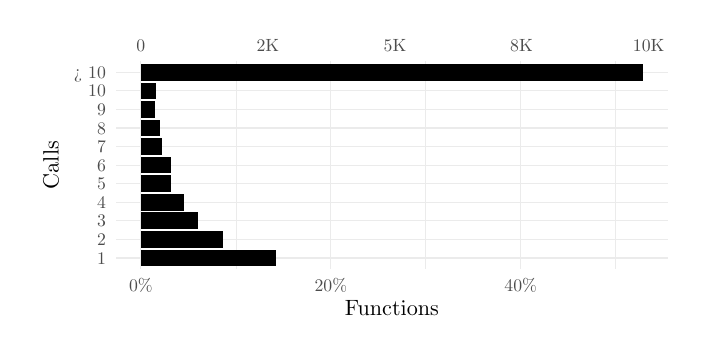
\begin{tikzpicture}[x=1pt,y=1pt]
\definecolor{fillColor}{RGB}{255,255,255}
\path[use as bounding box,fill=fillColor,fill opacity=0.00] (0,0) rectangle (238.49,108.41);
\begin{scope}
\path[clip] ( 31.86, 21.16) rectangle (231.38, 96.31);
\definecolor{drawColor}{gray}{0.92}

\path[draw=drawColor,line width= 0.2pt,line join=round] ( 75.23, 21.16) --
	( 75.23, 96.31);

\path[draw=drawColor,line width= 0.2pt,line join=round] (143.83, 21.16) --
	(143.83, 96.31);

\path[draw=drawColor,line width= 0.2pt,line join=round] (212.43, 21.16) --
	(212.43, 96.31);

\path[draw=drawColor,line width= 0.4pt,line join=round] ( 31.86, 25.19) --
	(231.38, 25.19);

\path[draw=drawColor,line width= 0.4pt,line join=round] ( 31.86, 31.90) --
	(231.38, 31.90);

\path[draw=drawColor,line width= 0.4pt,line join=round] ( 31.86, 38.61) --
	(231.38, 38.61);

\path[draw=drawColor,line width= 0.4pt,line join=round] ( 31.86, 45.32) --
	(231.38, 45.32);

\path[draw=drawColor,line width= 0.4pt,line join=round] ( 31.86, 52.03) --
	(231.38, 52.03);

\path[draw=drawColor,line width= 0.4pt,line join=round] ( 31.86, 58.73) --
	(231.38, 58.73);

\path[draw=drawColor,line width= 0.4pt,line join=round] ( 31.86, 65.44) --
	(231.38, 65.44);

\path[draw=drawColor,line width= 0.4pt,line join=round] ( 31.86, 72.15) --
	(231.38, 72.15);

\path[draw=drawColor,line width= 0.4pt,line join=round] ( 31.86, 78.86) --
	(231.38, 78.86);

\path[draw=drawColor,line width= 0.4pt,line join=round] ( 31.86, 85.57) --
	(231.38, 85.57);

\path[draw=drawColor,line width= 0.4pt,line join=round] ( 31.86, 92.28) --
	(231.38, 92.28);

\path[draw=drawColor,line width= 0.4pt,line join=round] ( 40.93, 21.16) --
	( 40.93, 96.31);

\path[draw=drawColor,line width= 0.4pt,line join=round] (109.53, 21.16) --
	(109.53, 96.31);

\path[draw=drawColor,line width= 0.4pt,line join=round] (178.13, 21.16) --
	(178.13, 96.31);
\definecolor{fillColor}{RGB}{0,0,0}

\path[fill=fillColor] ( 40.93, 89.26) rectangle (222.31, 95.30);

\path[fill=fillColor] ( 40.93, 22.17) rectangle ( 89.89, 28.21);

\path[fill=fillColor] ( 40.93, 28.88) rectangle ( 70.62, 34.92);

\path[fill=fillColor] ( 40.93, 35.59) rectangle ( 61.56, 41.63);

\path[fill=fillColor] ( 40.93, 42.30) rectangle ( 56.31, 48.34);

\path[fill=fillColor] ( 40.93, 55.72) rectangle ( 51.90, 61.75);

\path[fill=fillColor] ( 40.93, 49.01) rectangle ( 51.87, 55.04);

\path[fill=fillColor] ( 40.93, 62.43) rectangle ( 48.49, 68.46);

\path[fill=fillColor] ( 40.93, 69.13) rectangle ( 47.87, 75.17);

\path[fill=fillColor] ( 40.93, 82.55) rectangle ( 46.25, 88.59);

\path[fill=fillColor] ( 40.93, 75.84) rectangle ( 46.18, 81.88);
\end{scope}
\begin{scope}
\path[clip] (  0.00,  0.00) rectangle (238.49,108.41);
\definecolor{drawColor}{gray}{0.30}

\node[text=drawColor,anchor=base,inner sep=0pt, outer sep=0pt, scale=  0.64] at ( 40.85, 99.91) {0};

\node[text=drawColor,anchor=base,inner sep=0pt, outer sep=0pt, scale=  0.64] at ( 86.78, 99.91) {2K};

\node[text=drawColor,anchor=base,inner sep=0pt, outer sep=0pt, scale=  0.64] at (132.72, 99.91) {5K};

\node[text=drawColor,anchor=base,inner sep=0pt, outer sep=0pt, scale=  0.64] at (178.45, 99.91) {8K};

\node[text=drawColor,anchor=base,inner sep=0pt, outer sep=0pt, scale=  0.64] at (224.39, 99.91) {10K};
\end{scope}
\begin{scope}
\path[clip] (  0.00,  0.00) rectangle (238.49,108.41);
\definecolor{drawColor}{gray}{0.30}

\node[text=drawColor,anchor=base east,inner sep=0pt, outer sep=0pt, scale=  0.64] at ( 28.26, 22.98) {1};

\node[text=drawColor,anchor=base east,inner sep=0pt, outer sep=0pt, scale=  0.64] at ( 28.26, 29.69) {2};

\node[text=drawColor,anchor=base east,inner sep=0pt, outer sep=0pt, scale=  0.64] at ( 28.26, 36.40) {3};

\node[text=drawColor,anchor=base east,inner sep=0pt, outer sep=0pt, scale=  0.64] at ( 28.26, 43.11) {4};

\node[text=drawColor,anchor=base east,inner sep=0pt, outer sep=0pt, scale=  0.64] at ( 28.26, 49.82) {5};

\node[text=drawColor,anchor=base east,inner sep=0pt, outer sep=0pt, scale=  0.64] at ( 28.26, 56.53) {6};

\node[text=drawColor,anchor=base east,inner sep=0pt, outer sep=0pt, scale=  0.64] at ( 28.26, 63.24) {7};

\node[text=drawColor,anchor=base east,inner sep=0pt, outer sep=0pt, scale=  0.64] at ( 28.26, 69.95) {8};

\node[text=drawColor,anchor=base east,inner sep=0pt, outer sep=0pt, scale=  0.64] at ( 28.26, 76.66) {9};

\node[text=drawColor,anchor=base east,inner sep=0pt, outer sep=0pt, scale=  0.64] at ( 28.26, 83.37) {10};

\node[text=drawColor,anchor=base east,inner sep=0pt, outer sep=0pt, scale=  0.64] at ( 28.26, 90.08) {> 10};
\end{scope}
\begin{scope}
\path[clip] (  0.00,  0.00) rectangle (238.49,108.41);
\definecolor{drawColor}{gray}{0.30}

\node[text=drawColor,anchor=base,inner sep=0pt, outer sep=0pt, scale=  0.64] at ( 40.93, 13.15) {0{\%}};

\node[text=drawColor,anchor=base,inner sep=0pt, outer sep=0pt, scale=  0.64] at (109.53, 13.15) {20{\%}};

\node[text=drawColor,anchor=base,inner sep=0pt, outer sep=0pt, scale=  0.64] at (178.13, 13.15) {40{\%}};
\end{scope}
\begin{scope}
\path[clip] (  0.00,  0.00) rectangle (238.49,108.41);
\definecolor{drawColor}{RGB}{0,0,0}

\node[text=drawColor,anchor=base,inner sep=0pt, outer sep=0pt, scale=  0.80] at (131.62,  4.40) {Functions};
\end{scope}
\begin{scope}
\path[clip] (  0.00,  0.00) rectangle (238.49,108.41);
\definecolor{drawColor}{RGB}{0,0,0}

\node[text=drawColor,rotate= 90.00,anchor=base,inner sep=0pt, outer sep=0pt, scale=  0.80] at ( 11.20, 58.73) {Calls};
\end{scope}
\end{tikzpicture}

  \caption{Call Distribution}
  \label{fig:calldist}
\end{figure}

\noindent
These functions have a total of 67K parameter positions.
Figure~\ref{fig:paramdist} shows the distribution of parameters: 3\% functions
have none, 22\% have one parameter, and 5\% have over 10. There are 4 functions
with over 50 parameters, and the \texttt{ggplot2::theme} function has 95
parameters.

\begin{figure}[!h]  \centering
  % Created by tikzDevice version 0.12.3.1 on 2021-06-03 17:14:19
% !TEX encoding = UTF-8 Unicode
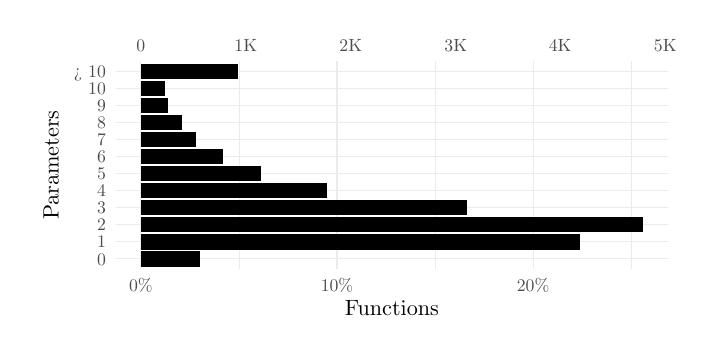
\begin{tikzpicture}[x=1pt,y=1pt]
\definecolor{fillColor}{RGB}{255,255,255}
\path[use as bounding box,fill=fillColor,fill opacity=0.00] (0,0) rectangle (238.49,108.41);
\begin{scope}
\path[clip] ( 31.86, 21.16) rectangle (231.38, 96.31);
\definecolor{drawColor}{gray}{0.92}

\path[draw=drawColor,line width= 0.2pt,line join=round] ( 76.35, 21.16) --
	( 76.35, 96.31);

\path[draw=drawColor,line width= 0.2pt,line join=round] (147.19, 21.16) --
	(147.19, 96.31);

\path[draw=drawColor,line width= 0.2pt,line join=round] (218.04, 21.16) --
	(218.04, 96.31);

\path[draw=drawColor,line width= 0.4pt,line join=round] ( 31.86, 24.86) --
	(231.38, 24.86);

\path[draw=drawColor,line width= 0.4pt,line join=round] ( 31.86, 31.02) --
	(231.38, 31.02);

\path[draw=drawColor,line width= 0.4pt,line join=round] ( 31.86, 37.18) --
	(231.38, 37.18);

\path[draw=drawColor,line width= 0.4pt,line join=round] ( 31.86, 43.34) --
	(231.38, 43.34);

\path[draw=drawColor,line width= 0.4pt,line join=round] ( 31.86, 49.50) --
	(231.38, 49.50);

\path[draw=drawColor,line width= 0.4pt,line join=round] ( 31.86, 55.66) --
	(231.38, 55.66);

\path[draw=drawColor,line width= 0.4pt,line join=round] ( 31.86, 61.81) --
	(231.38, 61.81);

\path[draw=drawColor,line width= 0.4pt,line join=round] ( 31.86, 67.97) --
	(231.38, 67.97);

\path[draw=drawColor,line width= 0.4pt,line join=round] ( 31.86, 74.13) --
	(231.38, 74.13);

\path[draw=drawColor,line width= 0.4pt,line join=round] ( 31.86, 80.29) --
	(231.38, 80.29);

\path[draw=drawColor,line width= 0.4pt,line join=round] ( 31.86, 86.45) --
	(231.38, 86.45);

\path[draw=drawColor,line width= 0.4pt,line join=round] ( 31.86, 92.61) --
	(231.38, 92.61);

\path[draw=drawColor,line width= 0.4pt,line join=round] ( 40.93, 21.16) --
	( 40.93, 96.31);

\path[draw=drawColor,line width= 0.4pt,line join=round] (111.77, 21.16) --
	(111.77, 96.31);

\path[draw=drawColor,line width= 0.4pt,line join=round] (182.62, 21.16) --
	(182.62, 96.31);
\definecolor{fillColor}{RGB}{0,0,0}

\path[fill=fillColor] ( 40.93, 89.84) rectangle ( 76.18, 95.38);

\path[fill=fillColor] ( 40.93, 22.09) rectangle ( 62.34, 27.63);

\path[fill=fillColor] ( 40.93, 28.25) rectangle (199.57, 33.79);

\path[fill=fillColor] ( 40.93, 83.68) rectangle ( 49.80, 89.22);

\path[fill=fillColor] ( 40.93, 34.41) rectangle (222.31, 39.95);

\path[fill=fillColor] ( 40.93, 40.56) rectangle (158.76, 46.11);

\path[fill=fillColor] ( 40.93, 46.72) rectangle (108.20, 52.27);

\path[fill=fillColor] ( 40.93, 52.88) rectangle ( 84.25, 58.43);

\path[fill=fillColor] ( 40.93, 59.04) rectangle ( 70.64, 64.59);

\path[fill=fillColor] ( 40.93, 65.20) rectangle ( 60.94, 70.75);

\path[fill=fillColor] ( 40.93, 71.36) rectangle ( 55.94, 76.91);

\path[fill=fillColor] ( 40.93, 77.52) rectangle ( 50.67, 83.06);
\end{scope}
\begin{scope}
\path[clip] (  0.00,  0.00) rectangle (238.49,108.41);
\definecolor{drawColor}{gray}{0.30}

\node[text=drawColor,anchor=base,inner sep=0pt, outer sep=0pt, scale=  0.64] at ( 40.85, 99.91) {0};

\node[text=drawColor,anchor=base,inner sep=0pt, outer sep=0pt, scale=  0.64] at ( 78.80, 99.91) {1K};

\node[text=drawColor,anchor=base,inner sep=0pt, outer sep=0pt, scale=  0.64] at (116.74, 99.91) {2K};

\node[text=drawColor,anchor=base,inner sep=0pt, outer sep=0pt, scale=  0.64] at (154.69, 99.91) {3K};

\node[text=drawColor,anchor=base,inner sep=0pt, outer sep=0pt, scale=  0.64] at (192.43, 99.91) {4K};

\node[text=drawColor,anchor=base,inner sep=0pt, outer sep=0pt, scale=  0.64] at (230.38, 99.91) {5K};
\end{scope}
\begin{scope}
\path[clip] (  0.00,  0.00) rectangle (238.49,108.41);
\definecolor{drawColor}{gray}{0.30}

\node[text=drawColor,anchor=base east,inner sep=0pt, outer sep=0pt, scale=  0.64] at ( 28.26, 22.65) {0};

\node[text=drawColor,anchor=base east,inner sep=0pt, outer sep=0pt, scale=  0.64] at ( 28.26, 28.81) {1};

\node[text=drawColor,anchor=base east,inner sep=0pt, outer sep=0pt, scale=  0.64] at ( 28.26, 34.97) {2};

\node[text=drawColor,anchor=base east,inner sep=0pt, outer sep=0pt, scale=  0.64] at ( 28.26, 41.13) {3};

\node[text=drawColor,anchor=base east,inner sep=0pt, outer sep=0pt, scale=  0.64] at ( 28.26, 47.29) {4};

\node[text=drawColor,anchor=base east,inner sep=0pt, outer sep=0pt, scale=  0.64] at ( 28.26, 53.45) {5};

\node[text=drawColor,anchor=base east,inner sep=0pt, outer sep=0pt, scale=  0.64] at ( 28.26, 59.61) {6};

\node[text=drawColor,anchor=base east,inner sep=0pt, outer sep=0pt, scale=  0.64] at ( 28.26, 65.77) {7};

\node[text=drawColor,anchor=base east,inner sep=0pt, outer sep=0pt, scale=  0.64] at ( 28.26, 71.93) {8};

\node[text=drawColor,anchor=base east,inner sep=0pt, outer sep=0pt, scale=  0.64] at ( 28.26, 78.09) {9};

\node[text=drawColor,anchor=base east,inner sep=0pt, outer sep=0pt, scale=  0.64] at ( 28.26, 84.25) {10};

\node[text=drawColor,anchor=base east,inner sep=0pt, outer sep=0pt, scale=  0.64] at ( 28.26, 90.41) {> 10};
\end{scope}
\begin{scope}
\path[clip] (  0.00,  0.00) rectangle (238.49,108.41);
\definecolor{drawColor}{gray}{0.30}

\node[text=drawColor,anchor=base,inner sep=0pt, outer sep=0pt, scale=  0.64] at ( 40.93, 13.15) {0{\%}};

\node[text=drawColor,anchor=base,inner sep=0pt, outer sep=0pt, scale=  0.64] at (111.77, 13.15) {10{\%}};

\node[text=drawColor,anchor=base,inner sep=0pt, outer sep=0pt, scale=  0.64] at (182.62, 13.15) {20{\%}};
\end{scope}
\begin{scope}
\path[clip] (  0.00,  0.00) rectangle (238.49,108.41);
\definecolor{drawColor}{RGB}{0,0,0}

\node[text=drawColor,anchor=base,inner sep=0pt, outer sep=0pt, scale=  0.80] at (131.62,  4.40) {Functions};
\end{scope}
\begin{scope}
\path[clip] (  0.00,  0.00) rectangle (238.49,108.41);
\definecolor{drawColor}{RGB}{0,0,0}

\node[text=drawColor,rotate= 90.00,anchor=base,inner sep=0pt, outer sep=0pt, scale=  0.80] at ( 11.20, 58.73) {Parameters};
\end{scope}
\end{tikzpicture}

  \caption{Parameter Distribution}
  \label{fig:paramdist}
\end{figure}

We counted \ObjCntEnvironment environments, which makes them the second most
widely allocated values. Table~\ref{table:object_count_dist} shows the frequency
of other values for comparison. Promises lead as there is one per
parameter~\cite{oopsla19b}. Vectors of logicals and characters are more frequent
than integers, reals, and raw.
Table~\ref{table:api_calls} gives the number of calls made to the various
environment APIs.


\begin{table}[!h]  \vspace{-3mm}  \small
  \caption{Object Counts} \label{table:object_count_dist}
  \centering
  \begin{tabular}{lr} \toprule
    \textbf{Type}&\textbf{Count}\\\midrule
    Promise&\ObjCntPromise\\
    Environment&\ObjCntEnvironment\\
    Logical&\ObjCntLogical\\
    Character&\ObjCntCharacter\\
    Language&\ObjCntLanguage\\
    Integer&\ObjCntInteger\\\bottomrule
  \end{tabular}
  \begin{tabular}{lr}\toprule
    \textbf{Type}&\textbf{Count}\\\midrule
    List&\ObjCntList\\
    Closure&\ObjCntClosure\\
    Real&\ObjCntReal\\
    Symbol&\ObjCntSymbol\\
    Raw&\ObjCntRaw\\
    Other&\ObjCntOther\\
    \bottomrule
  \end{tabular}
\end{table}


\begin{table*}[!h]
  \vspace{-3mm}
  \small
  \caption{API Calls} \label{table:api_calls}
  \centering
  \begin{tabular}{lr}
    \toprule
    \textbf{Function}&\textbf{Calls}\\
    \midrule
    \texttt{substitute}&\CallCntSubstitute\\
    \texttt{environment}&\CallCntEnvironment\\
    \texttt{baseenv}&\CallCntBaseenv\\
    \texttt{as.environment}&\CallCntAsDotenvironment\\
    \texttt{parent.frame}&\CallCntParentDotframe\\
    \texttt{getNamespace}&\CallCntGetnamespace\\
    \texttt{sys.frame}&\CallCntSysDotframe\\
    \texttt{get0}&\CallCntGetZero\\
    \texttt{get}&\CallCntGet\\
    \texttt{sys.parent}&\CallCntSysDotparent\\
    \texttt{[[}&\CallCntDBrack\\
    \bottomrule
  \end{tabular}
  \begin{tabular}{lr}
    \toprule
    \textbf{Function}&\textbf{Calls}\\
    \midrule
    \texttt{sys.function}&\CallCntSysDotfunction\\
    \texttt{list2env}&\CallCntListTwoenv\\
    \texttt{sys.call}&\CallCntSysDotcall\\
    \texttt{parent.env<-}&\CallCntParentDotenvAssign\\
    \texttt{parent.env}&\CallCntParentDotenv\\
    \texttt{\$}&\CallCntDollar\\
    \texttt{.subset2}&\CallCntDotSubsetTwo\\
    \texttt{sys.nframe}&\CallCntSysDotnframe\\
    \texttt{environment<-}&\CallCntEnvironmentAssign\\
    \texttt{\$<-}&\CallCntDollarAssign\\
    \texttt{exists}&\CallCntExists\\
    \bottomrule
  \end{tabular}
  \begin{tabular}{lr}
    \toprule
    \textbf{Function}&\textbf{Calls}\\
    \midrule
    \texttt{assign}&\CallCntAssign\\
    \texttt{lockBinding}&\CallCntLockbinding\\
    \texttt{mget}&\CallCntMget\\
    \texttt{emptyenv}&\CallCntEmptyenv\\
    \texttt{as.list}&\CallCntAsDotlist\\
    \texttt{lockEnvironment}&\CallCntLockenvironment\\
    \texttt{globalenv}&\CallCntGlobalenv\\
    \texttt{\~}&\CallCntTilde\\
    \texttt{environmentName}&\CallCntEnvironmentname\\
    \texttt{sys.calls}&\CallCntSysDotcalls\\
    \texttt{rm}&\CallCntRm\\
    \bottomrule
  \end{tabular}
  \begin{tabular}{lr}
    \toprule
    \textbf{Function}&\textbf{Calls}\\
    \midrule
    \texttt{[[<-}&\CallCntDBrackAssign\\
    \texttt{remove}&\CallCntRemove\\
    \texttt{sys.parents}&\CallCntSysDotparents\\
    \texttt{sys.frames}&\CallCntSysDotframes\\
    \texttt{dynGet}&\CallCntDynget\\
    \texttt{ls}&\CallCntLs\\
    \texttt{unlockBinding}&\CallCntUnlockbinding\\
    \texttt{length}&\CallCntLength\\
    \texttt{objects}&\CallCntObjects\\
    \texttt{pos.to.env}&\CallCntPosDottoDotenv\\
    \\
    \bottomrule
  \end{tabular}
\end{table*}


\section{Where do Environments come from?}

Table~\ref{table:env_source} presents the distribution of environments by
origin. The \emph{Core} row is for environments created by the language
implementation and the core 16 packages that ship with it.\footnote{They are
\code{base}, \code{compiler}, \code{datasets}, \code{grDevices},
\code{graphics}, \code{grid}, \code{methods}, \code{parallel}, \code{profile},
\code{splines}, \code{stats}, \code{stats4}, \code{tcltk}, \code{tools},
\code{translations}, and \code{utils.}} The \emph{User} row is for environments
that come from user-defined packages. We further differentiate between package
created in \emph{native} code and \emph{R} code. Native environments are created
using C APIs: \code{allocSExp}, \\\code{Rf_NewEnvironment}, and
\code{R_NewHashedEnv}. R environments come from calls to the \newEnv function.
Core is responsible for over 99\% of environments and this, mostly from C code.
Whereas the 0.03\% of User environment are twice as like to originate in R. We
encountered 904K environments which were unrelated to the code being traced.
They were created during the initialization of R session and were ignored from
the rest of the discussion.

\begin{table}[!h]
  \small
  \centering
  \caption{Environment Source}\label{table:env_source}
  \vspace{-3mm}
  \begin{tabular}{llrr}
    \toprule
    &\textbf{Source}&\textbf{\#}&\textbf{\%}\\
    \midrule
    \multirow{2}{*}{\textbf{Core}}  & \multicolumn{1}{l}{\emph{Native}} & \multicolumn{1}{r}{1.2B} & \multicolumn{1}{r}{99.62\%}\\
                                    & \multicolumn{1}{l}{\emph{R}}      & \multicolumn{1}{r}{3.1M} & \multicolumn{1}{r}{0.27\%}\\
    \midrule
    \multirow{2}{*}{\textbf{User}}  & \multicolumn{1}{l}{\emph{Native}} & \multicolumn{1}{r}{154.9K} & \multicolumn{1}{r}{0.01\%}\\
                                    & \multicolumn{1}{l}{\emph{R}}      & \multicolumn{1}{r}{240.4K} & \multicolumn{1}{r}{0.02\%}\\
    \bottomrule
  \end{tabular}
\end{table}

In the Core Native class, 99\% of environments are needed to implement function
environments. There 344K environment used for package namespaces, as well as
2.8M for the S4 object system implemented by the \code{methods} package. Some
165K were used for \c{eval} and 145K for \c{substitute}. In the Core R class,
94\% of the environments come from the \c{base} package and 5\% from
\code{methods}.


\section{How are Environment Used?}

We divide environments into three categories, presented in
Table~\ref{table:env_category}: \textbf{Calls} are environments used for
evaluating function calls, \textbf{Explicits} are created for non-standard
purposes, and \textbf{Packages} are needed for package loading.

\begin{table}[!h]
  \vspace{-3mm} \small
  \caption{Environment Categories} \label{table:env_category}
  \centering
  \begin{tabular}{lrr}    \toprule
    &\textbf{\#}&\textbf{\%}\\
    \midrule
    \textbf{Calls}&1.2B&99.3\%\\
    \textbf{Explicits}&3.7M&0.3\%\\
    \textbf{Packages}&3.3M&0.2\%\\ \bottomrule
  \end{tabular}
\end{table}


\subsection{Call Environments}

Of the 1.2B calls, only 20M environments are explicitly used by the functions in
Table~\ref{table:api_calls} The remaining environments are used implicitly for
reads and writes. To understand how the 20M environments are used, we look at
these events. The events of interest are described below.
\begin{itemize}
\item \texttt{A} for read, write and remove.
\item \texttt{V} for evaluating code in the environment using  \eval.
\item \texttt{S} for using \substitute in the environment.
\item \texttt{X} for extracting the environment using \code{parent.frame},
  \code{sys.frame} or \code{sys.frames}.
\end{itemize}

Table~\ref{table:call_env_seq} presents the frequency of the most common event
sets. Overall, there are 63 event sets but the top four sets explain the usage
patterns for 98\% of the call environments with any events. This is followed
by a long tail of event sets.

\begin{table}[!h]  \small
  \caption{Call Environment Events} \label{table:call_env_seq}  \centering
  \begin{tabular}{lrr}    \toprule
    \textbf{Event}&\textbf{\#}&\textbf{Cum. \%}\\
    \midrule
    \texttt{S}&          9.8M & 46\%\\
    \texttt{X, A}&       8.3M & 86\%\\
    \texttt{X, V, A}&    2.2M & 97\%\\
    \texttt{X, S, V, A}& 312K & 98\%\\
    \bottomrule
  \end{tabular}
\end{table}

\noindent
\textbf{S:} This event happens in functions that use \code{substitute}.
  Most of these cases originate from calls to \base package functions:
  \code{::}, \code{:::}, \code{delayedAssign}, and \code{evalq}. The expression
  \code{ns::sym} reads the value of publicly exported binding \code{sym} from
  namespace \code{ns}; \code{:::} also reads private bindings. These functions
  uses \substitute to access the symbol and namespace names, convert them to
  strings, and use the \code{get} function for the actual lookup. The
  \code{evalq} function is a variant of \eval. It uses the \substitute function
  to extract the expression AST for evaluation in a custom environment. The
  expression \code{delayedAssign(x, expr, eval_env, assign_env)} binds \code{x}
  to a promise containing the unevaluated expression \code{expr} in
  \code{assign_env}. The expression is evaluated in \code{eval_env}. The
  \code{expr} text is extracted using \code{substitute}.

\noindent
\textbf{X, A:} These events happen to function environments whose
  environment is extracted and used for accessing or modifying bindings. An
  example is the use of \code{delayedAssign} by
  \code{base::registerS3methods::assignWrapped} which uses \code{parent.frame}
  to extract the caller environment for evaluating promise code. Similarly,
  \code{withr::set_envvar} calls \code{base::match.arg} which also uses the
  parent environment. The \code{match.arg} function matches the argument text
  against a specified list of choices, provided as an argument. Another example
  is the \code{rlang::env_get} function which performs a lookup in the parent
  environment, extracted using \code{parent.frame}.

\noindent
\textbf{X, V, A:} These events happen when an environment is extracted
  and used for evaluating expressions. The use of \code{glue::glue} function by
  \code{waldo::path_attr} is one such example. The \code{glue::glue} function
  performs string interpolation by evaluating R code embedded in curly braces in
  a string. It extracts the caller's environment using \code{parent.frame},
  evaluates these embedded code blocks, and replaces them with their value to
  obtain the interpolated string. Another example is the \code{do.call}
  function, used by the \code{base::order} function. This function constructs a
  call expression with the supplied function name and arguments and evaluates it
  in the caller's environment, extracted using \code{parent.frame}.

\noindent
\textbf{X, S, V, A:} These events happen when an environment is used for
  \substitute as well as for evaluating expressions. This is particularly common
  in a code path of \code{match.arg} when the set of values against which the
  argument is to be matched are non provided. In this case, \code{match.arg}
  uses \code{substitute} to get the argument name, reflectively accesses its
  default value expression from the parent environment, and evaluates it to
  obtain the set of acceptable options. The \code{match.arg} function is used in
  this form in the \code{base::textConnection} function for matching string
  encoding. Another example is the \code{glue::glue_data} function. This
  function forms the core of the \code{glue::glue} function, doing the actual
  interpolation. It uses substitute to access the inputs, which could be unnamed
  strings to be interpolated, or named arguments to be made available for
  substitution. Then, it evaluates them using the \code{eval} function which
  extracts the environment using \code{parent.frame} for evaluation.


Apart from these sequences, formula construction also stands out as a relatively
frequent operation. These formulas extract the environment of the call in which
they are created and carry them around as attributes. We observed 66.6K formulas
constructed in call environments. The most common example is the
\code{stats::formula} function, which results in the creation of 11.2K formulas.
Apart from this, 2.8M call environments are used for evaluating code.


From this analysis, we conclude that most call environments do not have to be
explicit, since only 20M register any events. One would then expect an
optimizing compiler to optimize away accesses for these cases. Unfortunately, as
the event sets show, there are sufficient cases where environments are accessed
reflectively and the dynamic nature of R can make it challenging to predict when
this will happen. These environments can be passed around and modified at will,
making it hard to reason about the program from that point onwards. Especially
challenging is the use of the \code{eval} function on call environments, which
makes it possible to execute any code with arbitrary effects.

\subsection{Explicit Environments}
In this section, we discuss explicit environment creation using the \newEnv R
function and native code. 3.4M of these environments come from core and 395.2K
from user packages. We analyze the two environment categories below, separately.

\subsubsection{Core Environments}

There are 9 packages responsible for all the explicit environments from
\emph{Core}. Table~\ref{table:core_explicit_pack} shows the frequency of
environments they create. The \code{base} and \code{methods} packages alone
contribute to 99\% of the environments. The \code{base} package exports the
basic built-in functions of R and the \code{methods} package implements the S4
object-oriented system.

\begin{table}[!h]
  \small
  \caption{Core Explicit Environment Packages} \label{table:core_explicit_pack}
  \centering
  \begin{tabular}{lrr}
    \toprule
    \textbf{Package}&\textbf{\#}&\textbf{Cu. \%}\\
    \midrule
    \code{methods}&3.0M&89.2\%\\
    \code{base}&329.9K&99.0\%\\
    \code{grid}&15.7K&99.5\%\\
    \code{grDevices}&10.7K&99.8\%\\
    \code{stats}&2.7K&99.9\%\\
    \code{compiler}&2.4K&100\%\\
    \code{parallel}&610&100\%\\
    \code{tools}&217&100\%\\
    \code{utils}&7&100\%\\
    \bottomrule
  \end{tabular}
\end{table}

The explicit environments in these 9 packages originate from 60 functions.
Table~\ref{table:core_explicit_fun} shows the top 6 functions. These functions
alone contribute to 98\% of all the explicit environments in \emph{Core}. They
all belong to \code{methods} and \code{base} packages.

\begin{table}[!h]
  \small
  \caption{Core Explicit Environment Functions} \label{table:core_explicit_fun}
  \centering
  \begin{tabular}{lrr}
    \toprule
    \textbf{Function}&\textbf{\#}&\textbf{Cum. \%}\\
    \midrule
    \code{methods::new}&2.8M&84.3\%\\
    \code{base::eval}&165.5K&89.2\%\\
    \code{base::substitute}&145.8K&93.5\%\\
    \code{methods::.mlistAddToTable}&50.2K&95.0\%\\
    \code{methods::.resetInheritedMethods}&50.2K&96.5\%\\
    \code{methods::makeGeneric}&50.2K&98.0\%\\
    \bottomrule
  \end{tabular}
\end{table}

We now turn our attention to how these environments are used.
Table~\ref{table:core_explicit_env_seq} shows the top 5 of the total 27 event
sets. We observe three new events.
\begin{itemize}
\item \texttt{L} for locking the environment or its bindings
\item \texttt{Z} for modifying this environment's parent environment.
\item \texttt{!} for setting this environment as the parent of another
  environment or lexical scope of a function.
\end{itemize}

\begin{table}[!h]
  \small
  \caption{Core Explicit Environment Events} \label{table:core_explicit_env_seq}
  \centering
  \begin{tabular}{lrr}
    \toprule
    \textbf{Event}&\textbf{\#}&\textbf{Cum. \%}\\
    \midrule
    \texttt{A}&3.0M&88.4\%\\
    \texttt{A, V}&165.6K&93.4\%\\
    \texttt{S}&145.8K&97.7\%\\
    \texttt{A, Z, !}&50.2K&99.2\%\\
    \texttt{A, L, !}&12.1K&99.6\%\\
    \bottomrule
  \end{tabular}
\end{table}

\noindent
\textbf{A:} This is the most common pattern, and it occurs in many different
functions' environments. The most common example is the \code{methods::new}
function that is used for creating S4 objects. Another example is the
\code{grid} package that uses explicit environments to create viewport objects
and keys child viewports by name. The \code{parallel::addClusterOptions} function
uses an environment to store options such as port number, timeout, and R path
for the cluster used for parallel execution.

\noindent
\textbf{A, V:} This pattern represents environments created by the
\code{base::eval} and \code{base::evalq} functions. The default behavior of
these functions is to evaluate an expression in the supplied environment.
However, in these cases, a list of named elements is supplied instead of an
environment, which is internally converted into an environment for evaluation.

\noindent
\textbf{S:} This pattern comes from the \code{base::substitute} function. This
function is used for substituting symbols with expressions in ASTs. The
substitutions are usually read from an environment. However, in these cases,
lists are supplied instead; which are internally converted into environments.

\noindent
\textbf{A, Z, !:} This pattern comes from the methods package's
\code{makeGeneric} function. In the process of converting a function definition
to a generic function, it creates a new environment, assigns the field
\code{".Generic"} to the name of the generic method, sets its parent as the
lexical scope of the function (\texttt{Z}), and finally, sets the new
environment as the lexical scope of the function (\texttt{!}).

\noindent
\textbf{A, L, !:} These events happen in S4 objects. Their underlying data store
consists of an environment with a reference to the object. This binding is
locked to prevent modification.

Overall, 168.6K environments are passed to eval and only 100 were used for
formula construction.

Explicit environments in the \emph{Core} category are used for code evaluation,
substitution, and in the S4 object system. We find that these environments
register a variety of events. Their reliance on a significant proportion of R's
environment API makes these APIs crucial for the R ecosystem. Any efforts to
remove or simplify them will likely break all these packages.

\subsubsection{User Environments}

From our corpus, 55 packages are responsible for all the explicit environments
in the \emph{User} category. Table~\ref{table:user_explicit_pack} shows the
distribution of these environments by the top 8 packages, which account for
95.9\% of the environments in this category. The \code{vctrs} package provides
tools for type-coercion and size-recycling of R vectors. The \code{rlang}
package provides a consistent API to work with R objects and exposes an
evaluation mechanism used by the ``tidyverse'' packages for building DSLs.
\code{R6} implements a single-inheritance object-oriented system.
\code{codetools} implements code analysis for the R compiler. \code{ggplot2} is
a popular plotting library. \code{testthat} is widely used for testing R code.
The \code{dplyr} implements a DSL for SQL like queries on data frames.
Lastly, the \code{magrittr} package implements the pipe operator for building
function pipelines.

\begin{table}[!h]
  \small
  \caption{User Explicit Environment Packages} \label{table:user_explicit_pack}
  \centering
  \begin{tabular}{lrr}
    \toprule
    \textbf{Package}&\textbf{\#}&\textbf{Cu. \%}\\
    \midrule
    \code{vctrs}&142.9K&36.2\%\\
    \code{rlang}&75.2K&55.2\%\\
    \code{R6}&74.1K&73.9\%\\
    \code{codetools}&39.2K&83.8\%\\
    \code{ggplot2}&24.3K&90.0\%\\
    \code{testthat}&9.1K&92.3\%\\
    \code{dplyr}&8.3K&94.4\%\\
    \code{magrittr}&6.1K&95.9\%\\
    \bottomrule
  \end{tabular}
\end{table}

The explicit environments in these 55 packages originate from 322 functions.
Table~\ref{table:user_explicit_fun} shows the top ten functions. These functions
contribute to 65.1\% of all the explicit environments in \emph{User}. They
functions belong to 5 packages: \code{R6}, \code{vctrs}, \code{codetools},
\code{ggplot2}, and \code{rlang}.

\begin{table}[!h]
  \small
  \caption{User Explicit Environment Functions} \label{table:user_explicit_fun}
  \centering
  \begin{tabular}{lrr}
    \toprule
    \textbf{Function}&\textbf{\#}&\textbf{Cum. \%}\\
    \midrule
    \code{R6::generator_funs::new}&63.4K&16.0\%\\
    \code{vctrs::vec_c}&55.7K&30.1\%\\
    \code{codetools::mkHash}&31.3K&38.0\%\\
    \code{ggplot2::ggproto}&24.3K&44.2\%\\
    \code{rlang::eval_tidy}&18.1K&48.8\%\\
    \code{vctrs::vec_slice}&16.5K&52.9\%\\
    \code{rlang::new_data_mask}&13.8K&56.4\%\\
    \code{vctrs::vec_cast_common}&12.8K&59.7\%\\
    \code{vctrs::vec_as_names}&10.7K&62.4\%\\
    \code{R6::create_super_env}&10.6K&65.1\%\\
    \bottomrule
  \end{tabular}
\end{table}

Now, we turn our attention to how these environments are used.
Table~\ref{table:user_explicit_env_seq} shows the top 7 of the 82 event sets,
which characterize 96.5\% of these environments. We observe a new event,
\texttt{@}, used for setting the class attributes.

\begin{table}[!h]
  \small
  \caption{User Explicit Environment Events} \label{table:user_explicit_env_seq}
  \centering
  \begin{tabular}{lrr}
    \toprule
    \textbf{Events}&\textbf{\#}&\textbf{Cum. \%}\\
    \midrule
    \texttt{A, V}&154.0K&39.0\%\\
    \texttt{A}&102.8K&65.0\%\\
    \texttt{A, !}&43.8K&76.1\%\\
    \texttt{A, @}&38.9K&85.9\%\\
    \texttt{A, L}&30.4K&93.6\%\\
    \texttt{A, L, @}&8.3K&95.7\%\\
    \texttt{A, @, !}&3.2K&96.5\%\\
    \bottomrule
  \end{tabular}
\end{table}

\noindent
\textbf{A, V:} This set accounts for the majority of environments. It is
observed in 36 packages. These environments are created for custom evaluation
strategies, \ie, for evaluating expressions with custom bindings in the scope.
The \code{testthat} testing library uses custom environment for evaluating
testing code. The \code{vctrs::vec_c} function is an alternative to R's \code{c}
function for building a vector of values. It uses an explicit environment under
the hood for repairing the names of the vector elements. The
\code{rlang::eval_tidy} function is an alternative to R's \code{eval} which
provides support for evaluating ``quosures'', that are bundles of code and
environment. The \code{rlang} package creates three environments in native code
for use by its functions for evaluating expressions in the context of a data
frame.

\noindent
\textbf{A:} This pattern represents environments that are used as hash tables
and mutable state for packages. The \code{codetools} package provides facilities
for analysis of R code. Its \code{codetools::mkHash} function creates an
environment for use as a hash table to store intermediate static analysis
information. Another example is the \code{ps} package that provides facilities
for handling system processes. It uses an explicit environment for storing
package state such as error codes and socket types. The \code{iterators} package
uses environments as dynamic state of iterator objects.

\noindent
\textbf{A, !:} This pattern represents environments that are set as parents of
other environments or functions. This is dominated by \code{R.oo} and \code{R6}
packages that implement object-oriented systems. They create new environments
and set them as lexical scopes of object methods. Another example is the
\code{foreach} package which provides iteration constructs that can execute code
sequentially or in parallel. The \code{foreach::\%do\%} function creates a new
environment, assigns a marker, and sets it as the lexical scope of the function
which uses the marker to decide whether to execute the code in parallel or
sequentially.

\noindent
\textbf{A, @:} This pattern is used by packages to create custom objects, which
can be used for dispatch based on the class attribute of the environments.
\code{ggplot2} library implements \code{ggproto}, a prototype based
object-oriented system. The \code{ggproto} objects are explicit environments
with the \code{"ggproto"} class attribute. The \code{XML} package creates an
environment to store a tree of nodes and assigns it a class attribute. The
\code{xts} package creates a plot environment with plotting configuration and
sets a class attribute on it.

\noindent
\textbf{A, L:} This pattern shows up in the R6 package during object
instantiation. The private method bindings are locked in the object environment
to prevent any modification. Many calls to \code{lockBinding} also originate
form \code{data.table} which uses a custom environment to store intermediate
state for implementing data frame indexing.

\noindent
\textbf{A, L, @:} These events occur on environments from the \code{later} and
\code{R6} packages . The \code{later} package uses environments as handles for
event loop objects. These objects contain the unique loop identifier, which is
locked to prevent modification. The environments are then assigned the class
attribute, \code{"event_loop"}.

\noindent
\textbf{A, @, !:} This event pattern shows up on the environments from the
\code{plyr} package. This package creates environments with attribute
\code{"idf"} for representing immutable data frames. It also assigns getter
functions to these environments to access the columns of the data frame, and
sets their lexical scope to be the environment itself. The same pattern occurs
in \code{R6} when an environment representing a superclass object is set as the
parent environment of a subclass object environment.

Only 597 of the environments in this category were used for formula
construction. Out of these, 389 were created by the code being tested by
\code{testthat}. One example that stands out is the \code{survival} package
which creates explicit environments for use in formulas. We observe 22
environments created by \code{survival::coxph} and
\code{survival::model.frame.coxph} to be used for formula construction, as shown
below.

\begin{lstlisting}
coxenv <- new.env(parent= environment(formula))
assign("tt", function(x) x, envir=coxenv)
environment(tform$formula) <- coxenv
\end{lstlisting}

162K (41\%) of the explicit environments were used for dynamic code evaluation.
These environments were created from 33 packages. 88.2\% of these environments
were from the \code{vctrs} package. Four packages, \code{vctrs},
\code{testthat}, \code{magrittr}, and \code{rlang} together contribute 98.2\% of
these environments.

50.8K (12.9\%) of these environments have a class attribute.
Table~\ref{table:explicit_env_attr} presents the class attributes attached to
environments by frequency and the package from which the attributes originate.
\code{ggplot2} alone accounts for 47.8\% of environments, owing to the
\code{ggproto} object system. \code{ggplot2}, \code{rlang}, \code{R6}, and
\code{plyr} account for 99.2\% of the environments with attributes.
\begin{table}[!h]
  \small
  \caption{Environment Attributes} \label{table:explicit_env_attr}
  \centering
  \begin{tabular}{@{}ll@{}rr@{}}
    \toprule
    \textbf{Package}&\textbf{Attributes}&\textbf{\#}&\textbf{Cum. \%}\\
    \midrule
    \texttt{ggplot2}&\texttt{ggproto gg}&24.3K&47.8\%\\
    \texttt{rlang}&\texttt{rlang\_ctxt\_pronoun}&12.1K&71.5\%\\
    \texttt{R6}&\texttt{R6}&9.2K&89.5\%\\
    \texttt{rlang}&\texttt{r6lite}&3.7K&96.8\%\\
    \texttt{plyr}&\texttt{idf environment}&1.2K&99.2\%\\
    \texttt{later}&\texttt{event\_loop}&279&99.7\%\\
    \texttt{R6}&\texttt{R6ClassGenerator}&113&100\%\\
    \texttt{shiny}&\texttt{session\_proxy}&12&100\%\\
    \texttt{XML}&\texttt{XMLHashTree XMLAbstractDocument}&10.0&100\%\\
    \texttt{xts}&\texttt{replot\_xts environment}&2&100\%\\
    \bottomrule
  \end{tabular}
\end{table}

Environments in this category are used in a variety of ways. They are used as
hash tables, for customizing expression evaluation, and for designing custom
object systems. Attribute setting, environment locking, and modifying function's
local scopes are frequently occurring events for these environments. Any
modification to the corresponding environment APIs is likely to break these
packages.


\subsection{Package Environments}

We observe 3.3M environments related to packages and namespaces. The package
loading mechanism alone accounts for 2.9M of these environments. The remaining
environments are used as package namespaces. 2.3M of these environments
originate from a single \code{base} package function, \code{lazyLoadDBexec},
used only internally by R. This function is responsible for loading a package's
code from a binary file and also for loading processed help file data. A few
environments are created internally by the interpreter to store a package's
native functions for use by other packages. The namespace APIs of R are private,
and the internal structure of these environments is unspecified. It is also not
recommended to modify these environments. Hence, we don't capture events for
these environments.

\section{Enclosing Scope Manipulation}

A closure's enclosing scope can be accessed using \c{environment(fun)} and
modified using \c{environment(fun) <- env}. In this section, we look at the use
of these two APIs. Table~\ref{table:encl_scope_api} gives the calls to these two
functions. The table is missing \EnvAsnUnclassifiedCallPerc calls to
\c{environment<-} which could not be classified because of higher-order
functions, and dynamic behavior which prevented accurate name inference.

\begin{table}[!h]
  \small
  \centering
  \caption{Enclosing Scope API}\label{table:encl_scope_api}
  \vspace{-3mm}
  \begin{tabular}{llrrrr}
    \toprule &&\textbf{P\#}&\textbf{F\#}&\textbf{C\#}&\textbf{C\%}\\
    \midrule \multirow{2}{*}{\textbf{environment}}
             & \multicolumn{1}{l}{\emph{Core}} & \multicolumn{1}{r}{\EnvironmentCorePackCnt} & \multicolumn{1}{r}{\EnvironmentCoreFunCnt} & \multicolumn{1}{r}{\EnvironmentCoreCallCnt} & \multicolumn{1}{r}{\EnvironmentCoreCallPerc}\\
             & \multicolumn{1}{l}{\emph{User}} & \multicolumn{1}{r}{\EnvironmentUserPackCnt} & \multicolumn{1}{r}{\EnvironmentUserFunCnt} & \multicolumn{1}{r}{\EnvironmentUserCallCnt} & \multicolumn{1}{r}{\EnvironmentUserCallPerc}\\
    \midrule \multirow{2}{*}{\textbf{environment<-}}
             & \multicolumn{1}{l}{\emph{Core}} & \multicolumn{1}{r}{\EnvAsnCorePackCnt} & \multicolumn{1}{r}{\EnvAsnCoreFunCnt} & \multicolumn{1}{r}{\EnvAsnCoreCallCnt} & \multicolumn{1}{r}{\EnvAsnCoreCallPerc}\\
             & \multicolumn{1}{l}{\emph{User}} & \multicolumn{1}{r}{\EnvAsnUserPackCnt} & \multicolumn{1}{r}{\EnvAsnUserFunCnt} & \multicolumn{1}{r}{\EnvAsnUserCallCnt} & \multicolumn{1}{r}{\EnvAsnUserCallPerc}\\
    \bottomrule
  \end{tabular}
\end{table}

First, we look at the \c{environment} function. We observe that
\EnvironmentCoreCallPerc of the calls to \c{environment} originate from
\emph{Core}.

The \c{base::registerS3methods} is responsible for
\EnvironmentBaseRegisterMethodCallPerc calls to
\c{environment}. This function registers S3 methods for dispatch. It extracts
the enclosing environment of the method using \c{environment} (which is expected
to be the namespace environment) and updates the method information in its
\c{S3MethodsTable}.

The \c{methods} package functions are responsible for
\EnvironmentMethodsCallPerc calls. These functions perform introspection and
manipulation on the method environment as part of the object system
implementation.

The \c{compiler::cmpfun} function, used for byte code compilation of R
functions, is another client of \c{environment} function. It extracts the body,
formal parameter list, and the enclosing scope of the function to be compiled
(using \c{environment}) and passes them to a native function. Even though we
disable the byte code compiler for this study, we observe a few calls to this
function because it is explicitly called by testing scripts from the \c{rlang}
package.

The \c{utils::.defenv_for_S3_registry} function returns the top-level enclosing
scope of a function. It extracts the enclosing scope and walks over the parent
chain until it finds the package namespace in which the function was defined.

The \c{stats::ecdf} function computes an empirical cumulative distribution from
a numeric vector of observations. For this, it computes an approximation
function and assigns the number of observations in its environment (obtained
using \c{environment}) using the \c{assign} function.

Only, \EnvironmentUserCallPerc of the calls to \c{environment} originate from
\emph{User}. We discuss some of the patterns of usage below.

The \c{R.oo} package implements an Object-Oriented system. Its
\c{getStaticInstance.Class} function creates a static instance whose environment
is set to be the environment of the constructor function, obtained by calling
\c{environment}.

The \c{rlang} package implements \c{fn_env} function, which is a wrapper over
\c{environment}.

The \c{robustbase::mm} method takes a function as an argument and uses
c{environment} to extract its enclosing scope to look up a variable.

The \c{mgcv::fix.family.var} function returns a family of functions related to a
distribution. It retrieves the enclosing scope of the main function and sets it
as the enclosing scope of the other functions.

We observe that \c{environment<-} is called almost equally by both \emph{Core}
and \emph{User} packages. Table~\ref{table:env_asn_callers} gives the top five
callers of \c{environment<-}, which account for \EnvAsnTopFiveCallPerc calls.

\begin{table}[!h]
  \small
  \centering
  \caption{Top \c{environment<-} Callers}\label{table:env_asn_callers}
  \vspace{-3mm}
  \begin{tabular}{lr}
    \toprule \textbf{Function}&\textbf{Call \%}\\
    \midrule
    \EnvAsnOneCallerName&\EnvAsnOneCallPerc\\
    \EnvAsnTwoCallerName&\EnvAsnTwoCallPerc\\
    \EnvAsnThreeCallerName&\EnvAsnThreeCallPerc\\
    \EnvAsnFourCallerName&\EnvAsnFourCallPerc\\
    \EnvAsnFiveCallerName&\EnvAsnFiveCallPerc\\
    \bottomrule
  \end{tabular}
\end{table}

On the \c{Core} side, \c{methods}, and \c{stats} are responsible for all calls
to \c{environment<-}.

Two two functions of the \c{methods} package, \c{.makeDefaultBinding} and
\c{installClassMethod}, are responsible for \EnvAsnMethodsCallPerc of all
\c{Core} calls. These functions are used in the implementation of OOP-style
classes with reference semantics. The \c{.makeDefaultBinding} sets the
environment of a class method and \c{installClassMethod} sets a new environment
containing a reference to the superclass method as the environment of a method.

The \c{stats::make.link} function returns a list of functions related to a
model. These functions are defined as its inner functions which don't use any of
the parent scope bindings. Before returning, it modifies their definition
environment to be the \c{stats} package namespace.

On the \c{User} side, the \c{R6} package dominates the use of \c{environment<-}.
\EnvAsnOneCallerName is the most frequent caller, accounting for
\EnvAsnOneCallPerc of all calls. It uses \c{environment<-} to change the
enclosing scope of object methods.

A very common pattern for the use of \c{environment<-} is modifying the
environment of inner functions before returning them, similar to the
\c{stats::make.link} function, as shown below in the simplified definition of
\c{MASS::negative.binomial} function.

\begin{lstlisting}
negative.binomial <- function(theta) {
    env <- new.env(parent=.GlobalEnv);
    assign(".Theta", theta, envir=env);
    variance <- function(mu) mu + mu^2/.Theta
    environment(variance) <- env
    list(variance = variance, ...)
}

\end{lstlisting}

This pattern is exhibited by \EnvAsnUserInnerFunFunCnt functions from
\EnvAsnUserInnerFunPackCnt \emph{User} packages. Excluding \c{R6}, they make up
for \EnvAsnUserInnerFunCallPerc of the remaining \emph{User} calls to
\c{environment<-}. These functions are typically used for mathematical modeling.
They return a family of inner functions sharing common variables. To prevent
their own large environments from escaping, these functions create new
environments with the required bindings and set them as the scope of the
returned inner functions.

The \c{rlang::set_env} function implements a wrapper over \c{environment<-}.
This is only invoked from example programs in our corpus.

Another user of \c{environment<-} is the \c{foreach::\%do\%} function. It
modifies the environment of the currently registered parallel backend for
iteration. It inserts a new environment to the chain of parent environments of
the backend function containing a marker indicating whether the backend function
is called from \c{\%do\%}, or \c{\%dopar\%}.

\section{Locking and Unlocking}

In this section, we analyze the use of environment locking and unlocking APIs.
Locking an environment using \c{lockEnvironment} prevents the introduction of
new bindings. Locking individual bindings using \c{lockBinding} prevents their
mutation. An optional boolean argument to \c{lockEnvironment} also locks all the
existing bindings in the environment. Locked bindings can be unlocked for
mutation using \c{unlockEnvironment}. The use of this function triggers a
warning from the automated package checker (\c{R CMD check}), used by CRAN for
package submission. Table~\ref{lock_unlock_dist} presents the distribution of
calls to these three functions. For this discussion, we ignore the two
functions, \c{environmentIsLocked(env)} and \c{bindingIsLocked(sym, env)} used
for querying if the environment and binding are locked respectively.

\begin{table}[!h]
  \small
  \centering
  \caption{Locking and Unlocking API}\label{table:lock_unlock_dist}
  \vspace{-3mm}
  \begin{tabular}{llrrrr}
    \toprule &&\textbf{P\#}&\textbf{F\#}&\textbf{C\#}&\textbf{C\%}\\
    \midrule \multirow{2}{*}{\textbf{lockEnvironment}}
             & \multicolumn{1}{l}{\emph{Core}} & \multicolumn{1}{r}{\LockEnvironmentCorePackCnt} & \multicolumn{1}{r}{\LockEnvironmentCoreFunCnt} & \multicolumn{1}{r}{\LockEnvironmentCoreCallCnt} & \multicolumn{1}{r}{\LockEnvironmentCoreCallPerc}\\
             & \multicolumn{1}{l}{\emph{User}} & \multicolumn{1}{r}{\LockEnvironmentUserPackCnt} & \multicolumn{1}{r}{\LockEnvironmentUserFunCnt} & \multicolumn{1}{r}{\LockEnvironmentUserCallCnt} & \multicolumn{1}{r}{\LockEnvironmentUserCallPerc}\\
    \midrule \multirow{2}{*}{\textbf{lockBinding}}
             & \multicolumn{1}{l}{\emph{Core}} & \multicolumn{1}{r}{\LockBindingCorePackCnt} & \multicolumn{1}{r}{\LockBindingCoreFunCnt} & \multicolumn{1}{r}{\LockBindingCoreCallCnt} & \multicolumn{1}{r}{\LockBindingCoreCallPerc}\\
             & \multicolumn{1}{l}{\emph{User}} & \multicolumn{1}{r}{\LockBindingUserPackCnt} & \multicolumn{1}{r}{\LockBindingUserFunCnt} & \multicolumn{1}{r}{\LockBindingUserCallCnt} & \multicolumn{1}{r}{\LockBindingUserCallPerc}\\
    \midrule \multirow{2}{*}{\textbf{unlockBinding}}
             & \multicolumn{1}{l}{\emph{Core}} & \multicolumn{1}{r}{\UnlockBindingCorePackCnt} & \multicolumn{1}{r}{\UnlockBindingCoreFunCnt} & \multicolumn{1}{r}{\UnlockBindingCoreCallCnt} & \multicolumn{1}{r}{\UnlockBindingCoreCallPerc}\\
             & \multicolumn{1}{l}{\emph{User}} & \multicolumn{1}{r}{\UnlockBindingUserPackCnt} & \multicolumn{1}{r}{\UnlockBindingUserFunCnt} & \multicolumn{1}{r}{\UnlockBindingUserCallCnt} & \multicolumn{1}{r}{\UnlockBindingUserCallPerc}\\
    \bottomrule
  \end{tabular}
\end{table}

The \c{lockEnvironment} function is called \LockEnvironmentCoreCallPerc of the
times by three \c{base} package functions,
\c{base::loadNamespace::sealNamespace}, \c{base::attachNamespace}, and
\c{base::lazyLoadDBexec::envhook}. The first two functions are responsible for
initializing package and namespace environments. They are called with the
optional boolean argument set to \c{TRUE} to lock all the bindings in these
environments. \c{base::lazyLoadDBexec::envhook} function is used for loading
package code from a database.

On the \emph{User} side, only three functions from two packages, \c{R6} and
\c{rlang}, call \c{lockEnvironment}. The \c{rlang} package provides \c{env_lock}
function which is a wrapper for \c{lockEnvironment}. It was only called
\LockEnvironmentRlangCallCount times and all invocations were from test and
example scripts. The majority of calls originate from \c{R6}. The \c{R6::new}
functions calls \c{lockEnvironment} when creating new R6 class objects to lock
the environments used for public and private method bindings of the object.
\c{R6::clone} function calls \c{lockEnvironment} to lock the public and private
method environments of R6 object clones.

The \c{methods} package is responsible for all calls to \c{lockBinding} and
\c{unlockBinding} on the \emph{Core} side. These calls originate from private
methods, mostly to set fields in object environments.

On the \emph{User} side, the use of these functions is quite varied. Most
package functions call them in a matched pair. We discuss some interesting uses
below.

The \c{rJava} package uses JNI to implements a bridge between R and Java to
enable the creation and manipulation of Java objects from R. Its \c{.jinit}
method initializes the JVM upon invocation and caches references to basic Java
classes such as \c{Integer}, \c{Double}, etc. in its own namespace. Since all
the namespace bindings are locked by default, it unlocks the required bindings
using \c{unlockBinding}, updates them, and locks them again using
\c{lockBinding}.

The \c{gtools} package uses \c{lockBinding} and \c{unlockBinding} to circumvent
an
issue\footnote{\url{https://bugs.r-project.org/bugzilla/show_bug.cgi?id=15215}}
in the R VM. The R VM compiles package functions to bytecode during
installation, which is then interpreted using a bytecode interpreter. Calling
some functions in the \c{gtools} package causes the bytecode interpreter to run
out of stack space. To circumvent this problem, the package developers provide a
function, \c{unByteCodeAssign}, that updates the function binding in the package
namespace (by locking and unlocking the bindings) to an equivalent non-bytecode
version. The absence of bytecode forces the R VM to use an AST interpreter for
evaluation. The non-bytecode version of the function is obtained by reflectively
accessing the function's definition text and evaluating it to generate a new
function object with the same code and scope but without the bytecode.

The \c{[.data.table} implements subsetting for \c{data.table} objects. It
assigns the result of intermediate computation to a variable \c{.N} in caller's
environment, after copying its original value. It unlocks the binding first, if
needed, and locks it after restoring the original value of the variable. To
avoid warnings from automated package checker, this function calls
\c{unlockBinding} by passing it to \c{eval} as follows,
\c{eval(call("unlockBinding", ".N", parent.frame()))}.

The \c{igraph} package provides a progress bar for visualizing the progress of
its network analysis functions. It has a global progress bar object initialized
to \c{NULL} in the namespace environment. After package loading, the \c{igraph}
package uses \c{unlockBinding} to enable this binding to be mutated by its APIs
for updating their status.

The \c{rlang} package provides wrapper functions \c{env_binding_lock} and
\c{env_binding_unlock} for locking and unlocking environments. These functions
were only called from testing and example scripts in our corpus.

Finally, two \c{R6} functions, \c{new} and \c{clone} account for
\LockBindingRSixCallPerc of all calls to \c{lockBinding}. The \c{new} function
locks the methods in the private and public environments of the object. The
\c{generator_funs::clone_method} does the same to the object's clone. These
functions do not call \c{unlockBinding}.


We conclude that \c{R6} is the biggest user of the APIs discussed in this
section. Environment bindings are unlocked by very few functions, and they are
never used to inject new bindings or modify functions in other packages. We
found one instance of the use of \c{unlockBinding} to update the definitions of
\code{cbind} and \code{rbind} functions in the \code{base} package by
\code{data.table} prior to R version \texttt{4.0.0}. The dispatch behavior of
these functions prevented the correct overloaded method to be chosen when they
were called with two arguments of type \c{data.table} and \c{data.frame}
respectively. The \c{data.table} package modified these functions to address
this issue.


\section{Call Stack Reflection}

In this section, we analyze the use of APIs that enable reflective access to the
call-stack environments. Table~\ref{call_stack_ref} gives the distribution of
calls to these functions. \emph{Core} packages are the major users of
\c{parent.frame}, contributing to \ParentFrameCoreCallPerc calls. Though,
\emph{User} contributes to only \ParentFrameUserCallPerc calls, there are
\ParentFrameUserFunCnt clients of \c{parent.frame} from
\ParentFrameUserPackCnt packages.

\begin{table}[!h]
  \small
  \centering
  \caption{Call Stack Reflection API}\label{table:call_stack_ref}
  \vspace{-3mm}
  \begin{tabular}{llrrrr}
    \toprule &&\textbf{P\#}&\textbf{F\#}&\textbf{C\#}&\textbf{C\%}\\
    \midrule \multirow{2}{*}{\textbf{parent.frame}}
             & \multicolumn{1}{l}{\emph{Core}} & \multicolumn{1}{r}{\ParentFrameCorePackCnt} & \multicolumn{1}{r}{\ParentFrameCoreFunCnt} & \multicolumn{1}{r}{\ParentFrameCoreCallCnt} & \multicolumn{1}{r}{\ParentFrameCoreCallPerc}\\
             & \multicolumn{1}{l}{\emph{User}} & \multicolumn{1}{r}{\ParentFrameUserPackCnt} & \multicolumn{1}{r}{\ParentFrameUserFunCnt} & \multicolumn{1}{r}{\ParentFrameUserCallCnt} & \multicolumn{1}{r}{\ParentFrameUserCallPerc}\\
    \bottomrule
  \end{tabular}
\end{table}

Table~\ref{table:par_frm_top_core_callers} gives the list of top ten \c{Core} callers of
\c{parent.frame}. These callers make up for
\ParentFrameCoreTopTenCallPerc of all \emph{Core}.

\begin{table}[!h]
  \small
  \centering
  \caption{Top \c{parent.frame} \emph{Core} Callers}\label{table:par_frm_top_core_callers}
  \vspace{-3mm}
  \begin{tabular}{lr}
    \toprule \textbf{Function}&\textbf{Call \%}\\
    \midrule
    \ParentFrameCoreOneCallerName&\ParentFrameCoreOneCallPerc\\
    \ParentFrameCoreTwoCallerName&\ParentFrameCoreTwoCallPerc\\
    \ParentFrameCoreThreeCallerName&\ParentFrameCoreThreeCallPerc\\
    \ParentFrameCoreFourCallerName&\ParentFrameCoreFourCallPerc\\
    \ParentFrameCoreFiveCallerName&\ParentFrameCoreFiveCallPerc\\
    \ParentFrameCoreSixCallerName&\ParentFrameCoreSixCallPerc\\
    \ParentFrameCoreSevenCallerName&\ParentFrameCoreSevenCallPerc\\
    \ParentFrameCoreEightCallerName&\ParentFrameCoreEightCallPerc\\
    \ParentFrameCoreNineCallerName&\ParentFrameCoreNineCallPerc\\
    \ParentFrameCoreTenCallerName&\ParentFrameCoreTenCallPerc\\
    \bottomrule
  \end{tabular}
\end{table}

The \c{base::delayedAssign} function is the largest user of \c{parent.frame}.
This function is used to create a Promise from an unevaluated expression and
bind it to the specified variable. By default, it uses caller's environment
(extracted using \c{parent.frame}) as the evaluation environment for the
Promise's expression and the binding environment for the Promise object.

The \c{base::tryCatch} function evaluates the expression passed as argument in
caller's environment with handlers for catching exceptions.

The \c{base::match.call} function is used to reflectively access the call
expression with all argument names fully expanded (names of arguments can be
prefixes as long as they are not ambiguous). It uses \c{parent.frame(2} as the
environment to expand \c{...} (varargs) in the call expression.

The \c{base::match.fun} function is used for.

The \c{base::do.call} function constructs a call expression from a function name
and a list of arguments and evaluates it in the caller's environment unless a
different environment is explicitly specified.

The \c{base::eval} and \c{base::eval.parent} functions use \c{parent.frame} to
access the caller's and caller's caller's environments respectively for
evaluating expressions.

The \c{base::new.env} function creates a new environment and sets the caller's
environment as its parent environment.

Table~\ref{table:par_frm_top_user_callers} gives the list of top ten \c{User}
callers of \c{parent.frame}. These callers make up for
\ParentFrameUserTopTenCallPerc of all \emph{User} calls.

\begin{table}[!h]
  \small
  \centering
  \caption{Top \c{parent.frame} \emph{User} Callers}\label{table:par_frm_top_user_callers}
  \vspace{-3mm}
  \begin{tabular}{lr}
    \toprule \textbf{Function}&\textbf{Call \%}\\
    \midrule
    \ParentFrameUserOneCallerName&\ParentFrameUserOneCallPerc\\
    \ParentFrameUserTwoCallerName&\ParentFrameUserTwoCallPerc\\
    \ParentFrameUserThreeCallerName&\ParentFrameUserThreeCallPerc\\
    \ParentFrameUserFourCallerName&\ParentFrameUserFourCallPerc\\
    \ParentFrameUserFiveCallerName&\ParentFrameUserFiveCallPerc\\
    \ParentFrameUserSixCallerName&\ParentFrameUserSixCallPerc\\
    \ParentFrameUserSevenCallerName&\ParentFrameUserSevenCallPerc\\
    \ParentFrameUserEightCallerName&\ParentFrameUserEightCallPerc\\
    \ParentFrameUserNineCallerName&\ParentFrameUserNineCallPerc\\
    \ParentFrameUserTenCallerName&\ParentFrameUserTenCallPerc\\
    \bottomrule
  \end{tabular}
\end{table}

The \c{withr::defer} function allows attaching an expression to be evaluated
when exiting an active frame on the stack. It takes the frame environment as an
argument, which defaults to \c{parent.frame}. The \c{rlang::defer} function is a
copy of the \c{withr::defer}.

The \c{rlang::captureArgInfo} function is used for introspection of a binding in
an environment, which default to \c{parent.frame()}.

The \c{glue::glue} function


The argument \c{n} to \c{parent.frame} controls the number of frames to go back
in the call stack.

Passing \c{1} for \c{n} returns the environment of the caller. In our corpus,
\c{parent.frame} was called \ParentFrameDepthOneCallPerc of the times with \c{n}
as \c{1} by \ParentFrameDepthOneFunCnt functions. The top two callers are
\ParentFrameDepthOneCallerOneCallerName and
\ParentFrameDepthOneCallerTwoCallerName which account for
\ParentFrameDepthOneCallerOneCallPerc and \ParentFrameDepthOneCallerTwoCallPerc
of the calls in this category.

Next, \c{parent.frame} is invoked with the argument \c{2} by
\ParentFrameDepthTwoFunCnt functions which account for
\ParentFrameDepthTwoCallPerc of the calls. The top two callers are
\ParentFrameDepthTwoCallerOneCallerName and
\ParentFrameDepthTwoCallerTwoCallerName which account for
\ParentFrameDepthTwoCallerOneCallPerc and \ParentFrameDepthTwoCallerTwoCallPerc
of the calls in this category.

Finally, \ParentFrameDepthThreeCallPerc of the calls to \c{parent.frame}, made
from \ParentFrameDepthThreeFunCnt functions receive the argument \c{3}. The
first caller is \ParentFrameDepthThreeCallerOneCallerName which accounts for
\ParentFrameDepthThreeCallerOneCallPerc of the calls followed by
\ParentFrameDepthThreeCallerTwoCallerName which accounts for
\ParentFrameDepthThreeCallerTwoCallPerc of the calls.


\section{Conclusion}

This paper looked at first-class environments in R. We introduced the main
functions that operate on environments and reported on an observational study of
100 popular R packages. At the outset, our hope was that we could uncover some
ways to simplify and rationalize the design of R's environments. We conclude
with the rather disappointing observation that it seems that all of the
generality of the environment interface is needed, or at least that it is used.
While in the vast majority of cases environment access could be optimized and
environment could be implemented in a straightforward manner, there are
sufficient number of cases where environments escape and are used in a
reflective manner that it is not clear such optimizations can be widely applied.

In our future work, we plan to dig deeper into the data we have gathered and
identify particular patterns of usage that can be used by a compiler to predict
whether an environment will require full generality or if a more restricted
semantics could be applicable. As of this writing we do not know if this will
yield results.

\bibliography{bib/jv,bib/aviral}

\end{document}
